% Slides for talk on hydrogen fuel cells
% given in the department on October 27, 2003.
% 
% The original slides were in Prosper.  This file contains the
% translation of the original slides to Beamer.
% 
% Rouben Rostamian <rostamian@umbc.edu>
% August 31, 2004

\documentclass[CJK]{beamer}
%\usepackage{keynote-gradient} % Apple keynote theme

\usepackage{CJKutf8}  % for chinese
\usepackage{hyperref} % for url
\usepackage{pdfpages}
\hypersetup{colorlinks, linkcolor=blue, citecolor=blue,
    urlcolor=blue,
    plainpages=flase,
    pdfcreator=tex,
    bookmarksopen=true,
    pdfhighlight=/P,
    pdfstartview=FitH,
    pdfpagemode=UseOutlines,%UseOutlines, %None, FullScreen, UseThumbs
    pdfnewwindow % open pdf on another tab
}

\setbeamertemplate{frametitle}[default][center]

% beamer footnote
\usepackage[absolute,overlay]{textpos}
\newenvironment{reference}[2]{%
  \begin{textblock*}{\textwidth}(#1,#2)
      \footnotesize\it\bgroup\color{red!50!black}}{\egroup\end{textblock*}}


\usepackage{fancyvrb}
\usepackage{color}

\makeatletter
\def\PY@reset{\let\PY@it=\relax \let\PY@bf=\relax%
    \let\PY@ul=\relax \let\PY@tc=\relax%
    \let\PY@bc=\relax \let\PY@ff=\relax}
\def\PY@tok#1{\csname PY@tok@#1\endcsname}
\def\PY@toks#1+{\ifx\relax#1\empty\else%
    \PY@tok{#1}\expandafter\PY@toks\fi}
\def\PY@do#1{\PY@bc{\PY@tc{\PY@ul{%
    \PY@it{\PY@bf{\PY@ff{#1}}}}}}}
\def\PY#1#2{\PY@reset\PY@toks#1+\relax+\PY@do{#2}}

\expandafter\def\csname PY@tok@gd\endcsname{\def\PY@tc##1{\textcolor[rgb]{0.63,0.00,0.00}{##1}}}
\expandafter\def\csname PY@tok@gu\endcsname{\let\PY@bf=\textbf\def\PY@tc##1{\textcolor[rgb]{0.50,0.00,0.50}{##1}}}
\expandafter\def\csname PY@tok@gt\endcsname{\def\PY@tc##1{\textcolor[rgb]{0.00,0.27,0.87}{##1}}}
\expandafter\def\csname PY@tok@gs\endcsname{\let\PY@bf=\textbf}
\expandafter\def\csname PY@tok@gr\endcsname{\def\PY@tc##1{\textcolor[rgb]{1.00,0.00,0.00}{##1}}}
\expandafter\def\csname PY@tok@cm\endcsname{\let\PY@it=\textit\def\PY@tc##1{\textcolor[rgb]{0.25,0.50,0.50}{##1}}}
\expandafter\def\csname PY@tok@vg\endcsname{\def\PY@tc##1{\textcolor[rgb]{0.10,0.09,0.49}{##1}}}
\expandafter\def\csname PY@tok@m\endcsname{\def\PY@tc##1{\textcolor[rgb]{0.40,0.40,0.40}{##1}}}
\expandafter\def\csname PY@tok@mh\endcsname{\def\PY@tc##1{\textcolor[rgb]{0.40,0.40,0.40}{##1}}}
\expandafter\def\csname PY@tok@go\endcsname{\def\PY@tc##1{\textcolor[rgb]{0.53,0.53,0.53}{##1}}}
\expandafter\def\csname PY@tok@ge\endcsname{\let\PY@it=\textit}
\expandafter\def\csname PY@tok@vc\endcsname{\def\PY@tc##1{\textcolor[rgb]{0.10,0.09,0.49}{##1}}}
\expandafter\def\csname PY@tok@il\endcsname{\def\PY@tc##1{\textcolor[rgb]{0.40,0.40,0.40}{##1}}}
\expandafter\def\csname PY@tok@cs\endcsname{\let\PY@it=\textit\def\PY@tc##1{\textcolor[rgb]{0.25,0.50,0.50}{##1}}}
\expandafter\def\csname PY@tok@cp\endcsname{\def\PY@tc##1{\textcolor[rgb]{0.74,0.48,0.00}{##1}}}
\expandafter\def\csname PY@tok@gi\endcsname{\def\PY@tc##1{\textcolor[rgb]{0.00,0.63,0.00}{##1}}}
\expandafter\def\csname PY@tok@gh\endcsname{\let\PY@bf=\textbf\def\PY@tc##1{\textcolor[rgb]{0.00,0.00,0.50}{##1}}}
\expandafter\def\csname PY@tok@ni\endcsname{\let\PY@bf=\textbf\def\PY@tc##1{\textcolor[rgb]{0.60,0.60,0.60}{##1}}}
\expandafter\def\csname PY@tok@nl\endcsname{\def\PY@tc##1{\textcolor[rgb]{0.63,0.63,0.00}{##1}}}
\expandafter\def\csname PY@tok@nn\endcsname{\let\PY@bf=\textbf\def\PY@tc##1{\textcolor[rgb]{0.00,0.00,1.00}{##1}}}
\expandafter\def\csname PY@tok@no\endcsname{\def\PY@tc##1{\textcolor[rgb]{0.53,0.00,0.00}{##1}}}
\expandafter\def\csname PY@tok@na\endcsname{\def\PY@tc##1{\textcolor[rgb]{0.49,0.56,0.16}{##1}}}
\expandafter\def\csname PY@tok@nb\endcsname{\def\PY@tc##1{\textcolor[rgb]{0.00,0.50,0.00}{##1}}}
\expandafter\def\csname PY@tok@nc\endcsname{\let\PY@bf=\textbf\def\PY@tc##1{\textcolor[rgb]{0.00,0.00,1.00}{##1}}}
\expandafter\def\csname PY@tok@nd\endcsname{\def\PY@tc##1{\textcolor[rgb]{0.67,0.13,1.00}{##1}}}
\expandafter\def\csname PY@tok@ne\endcsname{\let\PY@bf=\textbf\def\PY@tc##1{\textcolor[rgb]{0.82,0.25,0.23}{##1}}}
\expandafter\def\csname PY@tok@nf\endcsname{\def\PY@tc##1{\textcolor[rgb]{0.00,0.00,1.00}{##1}}}
\expandafter\def\csname PY@tok@si\endcsname{\let\PY@bf=\textbf\def\PY@tc##1{\textcolor[rgb]{0.73,0.40,0.53}{##1}}}
\expandafter\def\csname PY@tok@s2\endcsname{\def\PY@tc##1{\textcolor[rgb]{0.73,0.13,0.13}{##1}}}
\expandafter\def\csname PY@tok@vi\endcsname{\def\PY@tc##1{\textcolor[rgb]{0.10,0.09,0.49}{##1}}}
\expandafter\def\csname PY@tok@nt\endcsname{\let\PY@bf=\textbf\def\PY@tc##1{\textcolor[rgb]{0.00,0.50,0.00}{##1}}}
\expandafter\def\csname PY@tok@nv\endcsname{\def\PY@tc##1{\textcolor[rgb]{0.10,0.09,0.49}{##1}}}
\expandafter\def\csname PY@tok@s1\endcsname{\def\PY@tc##1{\textcolor[rgb]{0.73,0.13,0.13}{##1}}}
\expandafter\def\csname PY@tok@sh\endcsname{\def\PY@tc##1{\textcolor[rgb]{0.73,0.13,0.13}{##1}}}
\expandafter\def\csname PY@tok@sc\endcsname{\def\PY@tc##1{\textcolor[rgb]{0.73,0.13,0.13}{##1}}}
\expandafter\def\csname PY@tok@sx\endcsname{\def\PY@tc##1{\textcolor[rgb]{0.00,0.50,0.00}{##1}}}
\expandafter\def\csname PY@tok@bp\endcsname{\def\PY@tc##1{\textcolor[rgb]{0.00,0.50,0.00}{##1}}}
\expandafter\def\csname PY@tok@c1\endcsname{\let\PY@it=\textit\def\PY@tc##1{\textcolor[rgb]{0.25,0.50,0.50}{##1}}}
\expandafter\def\csname PY@tok@kc\endcsname{\let\PY@bf=\textbf\def\PY@tc##1{\textcolor[rgb]{0.00,0.50,0.00}{##1}}}
\expandafter\def\csname PY@tok@c\endcsname{\let\PY@it=\textit\def\PY@tc##1{\textcolor[rgb]{0.25,0.50,0.50}{##1}}}
\expandafter\def\csname PY@tok@mf\endcsname{\def\PY@tc##1{\textcolor[rgb]{0.40,0.40,0.40}{##1}}}
\expandafter\def\csname PY@tok@err\endcsname{\def\PY@bc##1{\setlength{\fboxsep}{0pt}\fcolorbox[rgb]{1.00,0.00,0.00}{1,1,1}{\strut ##1}}}
\expandafter\def\csname PY@tok@kd\endcsname{\let\PY@bf=\textbf\def\PY@tc##1{\textcolor[rgb]{0.00,0.50,0.00}{##1}}}
\expandafter\def\csname PY@tok@ss\endcsname{\def\PY@tc##1{\textcolor[rgb]{0.10,0.09,0.49}{##1}}}
\expandafter\def\csname PY@tok@sr\endcsname{\def\PY@tc##1{\textcolor[rgb]{0.73,0.40,0.53}{##1}}}
\expandafter\def\csname PY@tok@mo\endcsname{\def\PY@tc##1{\textcolor[rgb]{0.40,0.40,0.40}{##1}}}
\expandafter\def\csname PY@tok@kn\endcsname{\let\PY@bf=\textbf\def\PY@tc##1{\textcolor[rgb]{0.00,0.50,0.00}{##1}}}
\expandafter\def\csname PY@tok@mi\endcsname{\def\PY@tc##1{\textcolor[rgb]{0.40,0.40,0.40}{##1}}}
\expandafter\def\csname PY@tok@gp\endcsname{\let\PY@bf=\textbf\def\PY@tc##1{\textcolor[rgb]{0.00,0.00,0.50}{##1}}}
\expandafter\def\csname PY@tok@o\endcsname{\def\PY@tc##1{\textcolor[rgb]{0.40,0.40,0.40}{##1}}}
\expandafter\def\csname PY@tok@kr\endcsname{\let\PY@bf=\textbf\def\PY@tc##1{\textcolor[rgb]{0.00,0.50,0.00}{##1}}}
\expandafter\def\csname PY@tok@s\endcsname{\def\PY@tc##1{\textcolor[rgb]{0.73,0.13,0.13}{##1}}}
\expandafter\def\csname PY@tok@kp\endcsname{\def\PY@tc##1{\textcolor[rgb]{0.00,0.50,0.00}{##1}}}
\expandafter\def\csname PY@tok@w\endcsname{\def\PY@tc##1{\textcolor[rgb]{0.73,0.73,0.73}{##1}}}
\expandafter\def\csname PY@tok@kt\endcsname{\def\PY@tc##1{\textcolor[rgb]{0.69,0.00,0.25}{##1}}}
\expandafter\def\csname PY@tok@ow\endcsname{\let\PY@bf=\textbf\def\PY@tc##1{\textcolor[rgb]{0.67,0.13,1.00}{##1}}}
\expandafter\def\csname PY@tok@sb\endcsname{\def\PY@tc##1{\textcolor[rgb]{0.73,0.13,0.13}{##1}}}
\expandafter\def\csname PY@tok@k\endcsname{\let\PY@bf=\textbf\def\PY@tc##1{\textcolor[rgb]{0.00,0.50,0.00}{##1}}}
\expandafter\def\csname PY@tok@se\endcsname{\let\PY@bf=\textbf\def\PY@tc##1{\textcolor[rgb]{0.73,0.40,0.13}{##1}}}
\expandafter\def\csname PY@tok@sd\endcsname{\let\PY@it=\textit\def\PY@tc##1{\textcolor[rgb]{0.73,0.13,0.13}{##1}}}

\def\PYZbs{\char`\\}
\def\PYZus{\char`\_}
\def\PYZob{\char`\{}
\def\PYZcb{\char`\}}
\def\PYZca{\char`\^}
\def\PYZam{\char`\&}
\def\PYZlt{\char`\<}
\def\PYZgt{\char`\>}
\def\PYZsh{\char`\#}
\def\PYZpc{\char`\%}
\def\PYZdl{\char`\$}
\def\PYZhy{\char`\-}
\def\PYZsq{\char`\'}
\def\PYZdq{\char`\"}
\def\PYZti{\char`\~}
% for compatibility with earlier versions
\def\PYZat{@}
\def\PYZlb{[}
\def\PYZrb{]}
\makeatother


\usepackage{fancyvrb}
\usepackage{color}



\makeatletter
\def\PY@reset{\let\PY@it=\relax \let\PY@bf=\relax%
    \let\PY@ul=\relax \let\PY@tc=\relax%
    \let\PY@bc=\relax \let\PY@ff=\relax}
\def\PY@tok#1{\csname PY@tok@#1\endcsname}
\def\PY@toks#1+{\ifx\relax#1\empty\else%
    \PY@tok{#1}\expandafter\PY@toks\fi}
\def\PY@do#1{\PY@bc{\PY@tc{\PY@ul{%
    \PY@it{\PY@bf{\PY@ff{#1}}}}}}}
\def\PY#1#2{\PY@reset\PY@toks#1+\relax+\PY@do{#2}}

\expandafter\def\csname PY@tok@gd\endcsname{\def\PY@tc##1{\textcolor[rgb]{0.63,0.00,0.00}{##1}}}
\expandafter\def\csname PY@tok@gu\endcsname{\let\PY@bf=\textbf\def\PY@tc##1{\textcolor[rgb]{0.50,0.00,0.50}{##1}}}
\expandafter\def\csname PY@tok@gt\endcsname{\def\PY@tc##1{\textcolor[rgb]{0.00,0.27,0.87}{##1}}}
\expandafter\def\csname PY@tok@gs\endcsname{\let\PY@bf=\textbf}
\expandafter\def\csname PY@tok@gr\endcsname{\def\PY@tc##1{\textcolor[rgb]{1.00,0.00,0.00}{##1}}}
\expandafter\def\csname PY@tok@cm\endcsname{\let\PY@it=\textit\def\PY@tc##1{\textcolor[rgb]{0.25,0.50,0.50}{##1}}}
\expandafter\def\csname PY@tok@vg\endcsname{\def\PY@tc##1{\textcolor[rgb]{0.10,0.09,0.49}{##1}}}
\expandafter\def\csname PY@tok@m\endcsname{\def\PY@tc##1{\textcolor[rgb]{0.40,0.40,0.40}{##1}}}
\expandafter\def\csname PY@tok@mh\endcsname{\def\PY@tc##1{\textcolor[rgb]{0.40,0.40,0.40}{##1}}}
\expandafter\def\csname PY@tok@go\endcsname{\def\PY@tc##1{\textcolor[rgb]{0.53,0.53,0.53}{##1}}}
\expandafter\def\csname PY@tok@ge\endcsname{\let\PY@it=\textit}
\expandafter\def\csname PY@tok@vc\endcsname{\def\PY@tc##1{\textcolor[rgb]{0.10,0.09,0.49}{##1}}}
\expandafter\def\csname PY@tok@il\endcsname{\def\PY@tc##1{\textcolor[rgb]{0.40,0.40,0.40}{##1}}}
\expandafter\def\csname PY@tok@cs\endcsname{\let\PY@it=\textit\def\PY@tc##1{\textcolor[rgb]{0.25,0.50,0.50}{##1}}}
\expandafter\def\csname PY@tok@cp\endcsname{\def\PY@tc##1{\textcolor[rgb]{0.74,0.48,0.00}{##1}}}
\expandafter\def\csname PY@tok@gi\endcsname{\def\PY@tc##1{\textcolor[rgb]{0.00,0.63,0.00}{##1}}}
\expandafter\def\csname PY@tok@gh\endcsname{\let\PY@bf=\textbf\def\PY@tc##1{\textcolor[rgb]{0.00,0.00,0.50}{##1}}}
\expandafter\def\csname PY@tok@ni\endcsname{\let\PY@bf=\textbf\def\PY@tc##1{\textcolor[rgb]{0.60,0.60,0.60}{##1}}}
\expandafter\def\csname PY@tok@nl\endcsname{\def\PY@tc##1{\textcolor[rgb]{0.63,0.63,0.00}{##1}}}
\expandafter\def\csname PY@tok@nn\endcsname{\let\PY@bf=\textbf\def\PY@tc##1{\textcolor[rgb]{0.00,0.00,1.00}{##1}}}
\expandafter\def\csname PY@tok@no\endcsname{\def\PY@tc##1{\textcolor[rgb]{0.53,0.00,0.00}{##1}}}
\expandafter\def\csname PY@tok@na\endcsname{\def\PY@tc##1{\textcolor[rgb]{0.49,0.56,0.16}{##1}}}
\expandafter\def\csname PY@tok@nb\endcsname{\def\PY@tc##1{\textcolor[rgb]{0.00,0.50,0.00}{##1}}}
\expandafter\def\csname PY@tok@nc\endcsname{\let\PY@bf=\textbf\def\PY@tc##1{\textcolor[rgb]{0.00,0.00,1.00}{##1}}}
\expandafter\def\csname PY@tok@nd\endcsname{\def\PY@tc##1{\textcolor[rgb]{0.67,0.13,1.00}{##1}}}
\expandafter\def\csname PY@tok@ne\endcsname{\let\PY@bf=\textbf\def\PY@tc##1{\textcolor[rgb]{0.82,0.25,0.23}{##1}}}
\expandafter\def\csname PY@tok@nf\endcsname{\def\PY@tc##1{\textcolor[rgb]{0.00,0.00,1.00}{##1}}}
\expandafter\def\csname PY@tok@si\endcsname{\let\PY@bf=\textbf\def\PY@tc##1{\textcolor[rgb]{0.73,0.40,0.53}{##1}}}
\expandafter\def\csname PY@tok@s2\endcsname{\def\PY@tc##1{\textcolor[rgb]{0.73,0.13,0.13}{##1}}}
\expandafter\def\csname PY@tok@vi\endcsname{\def\PY@tc##1{\textcolor[rgb]{0.10,0.09,0.49}{##1}}}
\expandafter\def\csname PY@tok@nt\endcsname{\let\PY@bf=\textbf\def\PY@tc##1{\textcolor[rgb]{0.00,0.50,0.00}{##1}}}
\expandafter\def\csname PY@tok@nv\endcsname{\def\PY@tc##1{\textcolor[rgb]{0.10,0.09,0.49}{##1}}}
\expandafter\def\csname PY@tok@s1\endcsname{\def\PY@tc##1{\textcolor[rgb]{0.73,0.13,0.13}{##1}}}
\expandafter\def\csname PY@tok@sh\endcsname{\def\PY@tc##1{\textcolor[rgb]{0.73,0.13,0.13}{##1}}}
\expandafter\def\csname PY@tok@sc\endcsname{\def\PY@tc##1{\textcolor[rgb]{0.73,0.13,0.13}{##1}}}
\expandafter\def\csname PY@tok@sx\endcsname{\def\PY@tc##1{\textcolor[rgb]{0.00,0.50,0.00}{##1}}}
\expandafter\def\csname PY@tok@bp\endcsname{\def\PY@tc##1{\textcolor[rgb]{0.00,0.50,0.00}{##1}}}
\expandafter\def\csname PY@tok@c1\endcsname{\let\PY@it=\textit\def\PY@tc##1{\textcolor[rgb]{0.25,0.50,0.50}{##1}}}
\expandafter\def\csname PY@tok@kc\endcsname{\let\PY@bf=\textbf\def\PY@tc##1{\textcolor[rgb]{0.00,0.50,0.00}{##1}}}
\expandafter\def\csname PY@tok@c\endcsname{\let\PY@it=\textit\def\PY@tc##1{\textcolor[rgb]{0.25,0.50,0.50}{##1}}}
\expandafter\def\csname PY@tok@mf\endcsname{\def\PY@tc##1{\textcolor[rgb]{0.40,0.40,0.40}{##1}}}
\expandafter\def\csname PY@tok@err\endcsname{\def\PY@bc##1{\setlength{\fboxsep}{0pt}\fcolorbox[rgb]{1.00,0.00,0.00}{1,1,1}{\strut ##1}}}
\expandafter\def\csname PY@tok@kd\endcsname{\let\PY@bf=\textbf\def\PY@tc##1{\textcolor[rgb]{0.00,0.50,0.00}{##1}}}
\expandafter\def\csname PY@tok@ss\endcsname{\def\PY@tc##1{\textcolor[rgb]{0.10,0.09,0.49}{##1}}}
\expandafter\def\csname PY@tok@sr\endcsname{\def\PY@tc##1{\textcolor[rgb]{0.73,0.40,0.53}{##1}}}
\expandafter\def\csname PY@tok@mo\endcsname{\def\PY@tc##1{\textcolor[rgb]{0.40,0.40,0.40}{##1}}}
\expandafter\def\csname PY@tok@kn\endcsname{\let\PY@bf=\textbf\def\PY@tc##1{\textcolor[rgb]{0.00,0.50,0.00}{##1}}}
\expandafter\def\csname PY@tok@mi\endcsname{\def\PY@tc##1{\textcolor[rgb]{0.40,0.40,0.40}{##1}}}
\expandafter\def\csname PY@tok@gp\endcsname{\let\PY@bf=\textbf\def\PY@tc##1{\textcolor[rgb]{0.00,0.00,0.50}{##1}}}
\expandafter\def\csname PY@tok@o\endcsname{\def\PY@tc##1{\textcolor[rgb]{0.40,0.40,0.40}{##1}}}
\expandafter\def\csname PY@tok@kr\endcsname{\let\PY@bf=\textbf\def\PY@tc##1{\textcolor[rgb]{0.00,0.50,0.00}{##1}}}
\expandafter\def\csname PY@tok@s\endcsname{\def\PY@tc##1{\textcolor[rgb]{0.73,0.13,0.13}{##1}}}
\expandafter\def\csname PY@tok@kp\endcsname{\def\PY@tc##1{\textcolor[rgb]{0.00,0.50,0.00}{##1}}}
\expandafter\def\csname PY@tok@w\endcsname{\def\PY@tc##1{\textcolor[rgb]{0.73,0.73,0.73}{##1}}}
\expandafter\def\csname PY@tok@kt\endcsname{\def\PY@tc##1{\textcolor[rgb]{0.69,0.00,0.25}{##1}}}
\expandafter\def\csname PY@tok@ow\endcsname{\let\PY@bf=\textbf\def\PY@tc##1{\textcolor[rgb]{0.67,0.13,1.00}{##1}}}
\expandafter\def\csname PY@tok@sb\endcsname{\def\PY@tc##1{\textcolor[rgb]{0.73,0.13,0.13}{##1}}}
\expandafter\def\csname PY@tok@k\endcsname{\let\PY@bf=\textbf\def\PY@tc##1{\textcolor[rgb]{0.00,0.50,0.00}{##1}}}
\expandafter\def\csname PY@tok@se\endcsname{\let\PY@bf=\textbf\def\PY@tc##1{\textcolor[rgb]{0.73,0.40,0.13}{##1}}}
\expandafter\def\csname PY@tok@sd\endcsname{\let\PY@it=\textit\def\PY@tc##1{\textcolor[rgb]{0.73,0.13,0.13}{##1}}}

\def\PYZbs{\char`\\}
\def\PYZus{\char`\_}
\def\PYZob{\char`\{}
\def\PYZcb{\char`\}}
\def\PYZca{\char`\^}
\def\PYZam{\char`\&}
\def\PYZlt{\char`\<}
\def\PYZgt{\char`\>}
\def\PYZsh{\char`\#}
\def\PYZpc{\char`\%}
\def\PYZdl{\char`\$}
\def\PYZhy{\char`\-}
\def\PYZsq{\char`\'}
\def\PYZdq{\char`\"}
\def\PYZti{\char`\~}
% for compatibility with earlier versions
\def\PYZat{@}
\def\PYZlb{[}
\def\PYZrb{]}
\makeatother


\usepackage{fancyvrb}
\usepackage{color}



\makeatletter
\def\PY@reset{\let\PY@it=\relax \let\PY@bf=\relax%
    \let\PY@ul=\relax \let\PY@tc=\relax%
    \let\PY@bc=\relax \let\PY@ff=\relax}
\def\PY@tok#1{\csname PY@tok@#1\endcsname}
\def\PY@toks#1+{\ifx\relax#1\empty\else%
    \PY@tok{#1}\expandafter\PY@toks\fi}
\def\PY@do#1{\PY@bc{\PY@tc{\PY@ul{%
    \PY@it{\PY@bf{\PY@ff{#1}}}}}}}
\def\PY#1#2{\PY@reset\PY@toks#1+\relax+\PY@do{#2}}

\expandafter\def\csname PY@tok@gd\endcsname{\def\PY@tc##1{\textcolor[rgb]{0.63,0.00,0.00}{##1}}}
\expandafter\def\csname PY@tok@gu\endcsname{\let\PY@bf=\textbf\def\PY@tc##1{\textcolor[rgb]{0.50,0.00,0.50}{##1}}}
\expandafter\def\csname PY@tok@gt\endcsname{\def\PY@tc##1{\textcolor[rgb]{0.00,0.27,0.87}{##1}}}
\expandafter\def\csname PY@tok@gs\endcsname{\let\PY@bf=\textbf}
\expandafter\def\csname PY@tok@gr\endcsname{\def\PY@tc##1{\textcolor[rgb]{1.00,0.00,0.00}{##1}}}
\expandafter\def\csname PY@tok@cm\endcsname{\let\PY@it=\textit\def\PY@tc##1{\textcolor[rgb]{0.25,0.50,0.50}{##1}}}
\expandafter\def\csname PY@tok@vg\endcsname{\def\PY@tc##1{\textcolor[rgb]{0.10,0.09,0.49}{##1}}}
\expandafter\def\csname PY@tok@m\endcsname{\def\PY@tc##1{\textcolor[rgb]{0.40,0.40,0.40}{##1}}}
\expandafter\def\csname PY@tok@mh\endcsname{\def\PY@tc##1{\textcolor[rgb]{0.40,0.40,0.40}{##1}}}
\expandafter\def\csname PY@tok@go\endcsname{\def\PY@tc##1{\textcolor[rgb]{0.53,0.53,0.53}{##1}}}
\expandafter\def\csname PY@tok@ge\endcsname{\let\PY@it=\textit}
\expandafter\def\csname PY@tok@vc\endcsname{\def\PY@tc##1{\textcolor[rgb]{0.10,0.09,0.49}{##1}}}
\expandafter\def\csname PY@tok@il\endcsname{\def\PY@tc##1{\textcolor[rgb]{0.40,0.40,0.40}{##1}}}
\expandafter\def\csname PY@tok@cs\endcsname{\let\PY@it=\textit\def\PY@tc##1{\textcolor[rgb]{0.25,0.50,0.50}{##1}}}
\expandafter\def\csname PY@tok@cp\endcsname{\def\PY@tc##1{\textcolor[rgb]{0.74,0.48,0.00}{##1}}}
\expandafter\def\csname PY@tok@gi\endcsname{\def\PY@tc##1{\textcolor[rgb]{0.00,0.63,0.00}{##1}}}
\expandafter\def\csname PY@tok@gh\endcsname{\let\PY@bf=\textbf\def\PY@tc##1{\textcolor[rgb]{0.00,0.00,0.50}{##1}}}
\expandafter\def\csname PY@tok@ni\endcsname{\let\PY@bf=\textbf\def\PY@tc##1{\textcolor[rgb]{0.60,0.60,0.60}{##1}}}
\expandafter\def\csname PY@tok@nl\endcsname{\def\PY@tc##1{\textcolor[rgb]{0.63,0.63,0.00}{##1}}}
\expandafter\def\csname PY@tok@nn\endcsname{\let\PY@bf=\textbf\def\PY@tc##1{\textcolor[rgb]{0.00,0.00,1.00}{##1}}}
\expandafter\def\csname PY@tok@no\endcsname{\def\PY@tc##1{\textcolor[rgb]{0.53,0.00,0.00}{##1}}}
\expandafter\def\csname PY@tok@na\endcsname{\def\PY@tc##1{\textcolor[rgb]{0.49,0.56,0.16}{##1}}}
\expandafter\def\csname PY@tok@nb\endcsname{\def\PY@tc##1{\textcolor[rgb]{0.00,0.50,0.00}{##1}}}
\expandafter\def\csname PY@tok@nc\endcsname{\let\PY@bf=\textbf\def\PY@tc##1{\textcolor[rgb]{0.00,0.00,1.00}{##1}}}
\expandafter\def\csname PY@tok@nd\endcsname{\def\PY@tc##1{\textcolor[rgb]{0.67,0.13,1.00}{##1}}}
\expandafter\def\csname PY@tok@ne\endcsname{\let\PY@bf=\textbf\def\PY@tc##1{\textcolor[rgb]{0.82,0.25,0.23}{##1}}}
\expandafter\def\csname PY@tok@nf\endcsname{\def\PY@tc##1{\textcolor[rgb]{0.00,0.00,1.00}{##1}}}
\expandafter\def\csname PY@tok@si\endcsname{\let\PY@bf=\textbf\def\PY@tc##1{\textcolor[rgb]{0.73,0.40,0.53}{##1}}}
\expandafter\def\csname PY@tok@s2\endcsname{\def\PY@tc##1{\textcolor[rgb]{0.73,0.13,0.13}{##1}}}
\expandafter\def\csname PY@tok@vi\endcsname{\def\PY@tc##1{\textcolor[rgb]{0.10,0.09,0.49}{##1}}}
\expandafter\def\csname PY@tok@nt\endcsname{\let\PY@bf=\textbf\def\PY@tc##1{\textcolor[rgb]{0.00,0.50,0.00}{##1}}}
\expandafter\def\csname PY@tok@nv\endcsname{\def\PY@tc##1{\textcolor[rgb]{0.10,0.09,0.49}{##1}}}
\expandafter\def\csname PY@tok@s1\endcsname{\def\PY@tc##1{\textcolor[rgb]{0.73,0.13,0.13}{##1}}}
\expandafter\def\csname PY@tok@sh\endcsname{\def\PY@tc##1{\textcolor[rgb]{0.73,0.13,0.13}{##1}}}
\expandafter\def\csname PY@tok@sc\endcsname{\def\PY@tc##1{\textcolor[rgb]{0.73,0.13,0.13}{##1}}}
\expandafter\def\csname PY@tok@sx\endcsname{\def\PY@tc##1{\textcolor[rgb]{0.00,0.50,0.00}{##1}}}
\expandafter\def\csname PY@tok@bp\endcsname{\def\PY@tc##1{\textcolor[rgb]{0.00,0.50,0.00}{##1}}}
\expandafter\def\csname PY@tok@c1\endcsname{\let\PY@it=\textit\def\PY@tc##1{\textcolor[rgb]{0.25,0.50,0.50}{##1}}}
\expandafter\def\csname PY@tok@kc\endcsname{\let\PY@bf=\textbf\def\PY@tc##1{\textcolor[rgb]{0.00,0.50,0.00}{##1}}}
\expandafter\def\csname PY@tok@c\endcsname{\let\PY@it=\textit\def\PY@tc##1{\textcolor[rgb]{0.25,0.50,0.50}{##1}}}
\expandafter\def\csname PY@tok@mf\endcsname{\def\PY@tc##1{\textcolor[rgb]{0.40,0.40,0.40}{##1}}}
\expandafter\def\csname PY@tok@err\endcsname{\def\PY@bc##1{\setlength{\fboxsep}{0pt}\fcolorbox[rgb]{1.00,0.00,0.00}{1,1,1}{\strut ##1}}}
\expandafter\def\csname PY@tok@kd\endcsname{\let\PY@bf=\textbf\def\PY@tc##1{\textcolor[rgb]{0.00,0.50,0.00}{##1}}}
\expandafter\def\csname PY@tok@ss\endcsname{\def\PY@tc##1{\textcolor[rgb]{0.10,0.09,0.49}{##1}}}
\expandafter\def\csname PY@tok@sr\endcsname{\def\PY@tc##1{\textcolor[rgb]{0.73,0.40,0.53}{##1}}}
\expandafter\def\csname PY@tok@mo\endcsname{\def\PY@tc##1{\textcolor[rgb]{0.40,0.40,0.40}{##1}}}
\expandafter\def\csname PY@tok@kn\endcsname{\let\PY@bf=\textbf\def\PY@tc##1{\textcolor[rgb]{0.00,0.50,0.00}{##1}}}
\expandafter\def\csname PY@tok@mi\endcsname{\def\PY@tc##1{\textcolor[rgb]{0.40,0.40,0.40}{##1}}}
\expandafter\def\csname PY@tok@gp\endcsname{\let\PY@bf=\textbf\def\PY@tc##1{\textcolor[rgb]{0.00,0.00,0.50}{##1}}}
\expandafter\def\csname PY@tok@o\endcsname{\def\PY@tc##1{\textcolor[rgb]{0.40,0.40,0.40}{##1}}}
\expandafter\def\csname PY@tok@kr\endcsname{\let\PY@bf=\textbf\def\PY@tc##1{\textcolor[rgb]{0.00,0.50,0.00}{##1}}}
\expandafter\def\csname PY@tok@s\endcsname{\def\PY@tc##1{\textcolor[rgb]{0.73,0.13,0.13}{##1}}}
\expandafter\def\csname PY@tok@kp\endcsname{\def\PY@tc##1{\textcolor[rgb]{0.00,0.50,0.00}{##1}}}
\expandafter\def\csname PY@tok@w\endcsname{\def\PY@tc##1{\textcolor[rgb]{0.73,0.73,0.73}{##1}}}
\expandafter\def\csname PY@tok@kt\endcsname{\def\PY@tc##1{\textcolor[rgb]{0.69,0.00,0.25}{##1}}}
\expandafter\def\csname PY@tok@ow\endcsname{\let\PY@bf=\textbf\def\PY@tc##1{\textcolor[rgb]{0.67,0.13,1.00}{##1}}}
\expandafter\def\csname PY@tok@sb\endcsname{\def\PY@tc##1{\textcolor[rgb]{0.73,0.13,0.13}{##1}}}
\expandafter\def\csname PY@tok@k\endcsname{\let\PY@bf=\textbf\def\PY@tc##1{\textcolor[rgb]{0.00,0.50,0.00}{##1}}}
\expandafter\def\csname PY@tok@se\endcsname{\let\PY@bf=\textbf\def\PY@tc##1{\textcolor[rgb]{0.73,0.40,0.13}{##1}}}
\expandafter\def\csname PY@tok@sd\endcsname{\let\PY@it=\textit\def\PY@tc##1{\textcolor[rgb]{0.73,0.13,0.13}{##1}}}

\def\PYZbs{\char`\\}
\def\PYZus{\char`\_}
\def\PYZob{\char`\{}
\def\PYZcb{\char`\}}
\def\PYZca{\char`\^}
\def\PYZam{\char`\&}
\def\PYZlt{\char`\<}
\def\PYZgt{\char`\>}
\def\PYZsh{\char`\#}
\def\PYZpc{\char`\%}
\def\PYZdl{\char`\$}
\def\PYZhy{\char`\-}
\def\PYZsq{\char`\'}
\def\PYZdq{\char`\"}
\def\PYZti{\char`\~}
% for compatibility with earlier versions
\def\PYZat{@}
\def\PYZlb{[}
\def\PYZrb{]}
\makeatother


\usepackage{fancyvrb}
\usepackage{color}

\makeatletter
\def\PY@reset{\let\PY@it=\relax \let\PY@bf=\relax%
    \let\PY@ul=\relax \let\PY@tc=\relax%
    \let\PY@bc=\relax \let\PY@ff=\relax}
\def\PY@tok#1{\csname PY@tok@#1\endcsname}
\def\PY@toks#1+{\ifx\relax#1\empty\else%
    \PY@tok{#1}\expandafter\PY@toks\fi}
\def\PY@do#1{\PY@bc{\PY@tc{\PY@ul{%
    \PY@it{\PY@bf{\PY@ff{#1}}}}}}}
\def\PY#1#2{\PY@reset\PY@toks#1+\relax+\PY@do{#2}}

\expandafter\def\csname PY@tok@gd\endcsname{\def\PY@tc##1{\textcolor[rgb]{0.63,0.00,0.00}{##1}}}
\expandafter\def\csname PY@tok@gu\endcsname{\let\PY@bf=\textbf\def\PY@tc##1{\textcolor[rgb]{0.50,0.00,0.50}{##1}}}
\expandafter\def\csname PY@tok@gt\endcsname{\def\PY@tc##1{\textcolor[rgb]{0.00,0.27,0.87}{##1}}}
\expandafter\def\csname PY@tok@gs\endcsname{\let\PY@bf=\textbf}
\expandafter\def\csname PY@tok@gr\endcsname{\def\PY@tc##1{\textcolor[rgb]{1.00,0.00,0.00}{##1}}}
\expandafter\def\csname PY@tok@cm\endcsname{\let\PY@it=\textit\def\PY@tc##1{\textcolor[rgb]{0.25,0.50,0.50}{##1}}}
\expandafter\def\csname PY@tok@vg\endcsname{\def\PY@tc##1{\textcolor[rgb]{0.10,0.09,0.49}{##1}}}
\expandafter\def\csname PY@tok@m\endcsname{\def\PY@tc##1{\textcolor[rgb]{0.40,0.40,0.40}{##1}}}
\expandafter\def\csname PY@tok@mh\endcsname{\def\PY@tc##1{\textcolor[rgb]{0.40,0.40,0.40}{##1}}}
\expandafter\def\csname PY@tok@go\endcsname{\def\PY@tc##1{\textcolor[rgb]{0.53,0.53,0.53}{##1}}}
\expandafter\def\csname PY@tok@ge\endcsname{\let\PY@it=\textit}
\expandafter\def\csname PY@tok@vc\endcsname{\def\PY@tc##1{\textcolor[rgb]{0.10,0.09,0.49}{##1}}}
\expandafter\def\csname PY@tok@il\endcsname{\def\PY@tc##1{\textcolor[rgb]{0.40,0.40,0.40}{##1}}}
\expandafter\def\csname PY@tok@cs\endcsname{\let\PY@it=\textit\def\PY@tc##1{\textcolor[rgb]{0.25,0.50,0.50}{##1}}}
\expandafter\def\csname PY@tok@cp\endcsname{\def\PY@tc##1{\textcolor[rgb]{0.74,0.48,0.00}{##1}}}
\expandafter\def\csname PY@tok@gi\endcsname{\def\PY@tc##1{\textcolor[rgb]{0.00,0.63,0.00}{##1}}}
\expandafter\def\csname PY@tok@gh\endcsname{\let\PY@bf=\textbf\def\PY@tc##1{\textcolor[rgb]{0.00,0.00,0.50}{##1}}}
\expandafter\def\csname PY@tok@ni\endcsname{\let\PY@bf=\textbf\def\PY@tc##1{\textcolor[rgb]{0.60,0.60,0.60}{##1}}}
\expandafter\def\csname PY@tok@nl\endcsname{\def\PY@tc##1{\textcolor[rgb]{0.63,0.63,0.00}{##1}}}
\expandafter\def\csname PY@tok@nn\endcsname{\let\PY@bf=\textbf\def\PY@tc##1{\textcolor[rgb]{0.00,0.00,1.00}{##1}}}
\expandafter\def\csname PY@tok@no\endcsname{\def\PY@tc##1{\textcolor[rgb]{0.53,0.00,0.00}{##1}}}
\expandafter\def\csname PY@tok@na\endcsname{\def\PY@tc##1{\textcolor[rgb]{0.49,0.56,0.16}{##1}}}
\expandafter\def\csname PY@tok@nb\endcsname{\def\PY@tc##1{\textcolor[rgb]{0.00,0.50,0.00}{##1}}}
\expandafter\def\csname PY@tok@nc\endcsname{\let\PY@bf=\textbf\def\PY@tc##1{\textcolor[rgb]{0.00,0.00,1.00}{##1}}}
\expandafter\def\csname PY@tok@nd\endcsname{\def\PY@tc##1{\textcolor[rgb]{0.67,0.13,1.00}{##1}}}
\expandafter\def\csname PY@tok@ne\endcsname{\let\PY@bf=\textbf\def\PY@tc##1{\textcolor[rgb]{0.82,0.25,0.23}{##1}}}
\expandafter\def\csname PY@tok@nf\endcsname{\def\PY@tc##1{\textcolor[rgb]{0.00,0.00,1.00}{##1}}}
\expandafter\def\csname PY@tok@si\endcsname{\let\PY@bf=\textbf\def\PY@tc##1{\textcolor[rgb]{0.73,0.40,0.53}{##1}}}
\expandafter\def\csname PY@tok@s2\endcsname{\def\PY@tc##1{\textcolor[rgb]{0.73,0.13,0.13}{##1}}}
\expandafter\def\csname PY@tok@vi\endcsname{\def\PY@tc##1{\textcolor[rgb]{0.10,0.09,0.49}{##1}}}
\expandafter\def\csname PY@tok@nt\endcsname{\let\PY@bf=\textbf\def\PY@tc##1{\textcolor[rgb]{0.00,0.50,0.00}{##1}}}
\expandafter\def\csname PY@tok@nv\endcsname{\def\PY@tc##1{\textcolor[rgb]{0.10,0.09,0.49}{##1}}}
\expandafter\def\csname PY@tok@s1\endcsname{\def\PY@tc##1{\textcolor[rgb]{0.73,0.13,0.13}{##1}}}
\expandafter\def\csname PY@tok@sh\endcsname{\def\PY@tc##1{\textcolor[rgb]{0.73,0.13,0.13}{##1}}}
\expandafter\def\csname PY@tok@sc\endcsname{\def\PY@tc##1{\textcolor[rgb]{0.73,0.13,0.13}{##1}}}
\expandafter\def\csname PY@tok@sx\endcsname{\def\PY@tc##1{\textcolor[rgb]{0.00,0.50,0.00}{##1}}}
\expandafter\def\csname PY@tok@bp\endcsname{\def\PY@tc##1{\textcolor[rgb]{0.00,0.50,0.00}{##1}}}
\expandafter\def\csname PY@tok@c1\endcsname{\let\PY@it=\textit\def\PY@tc##1{\textcolor[rgb]{0.25,0.50,0.50}{##1}}}
\expandafter\def\csname PY@tok@kc\endcsname{\let\PY@bf=\textbf\def\PY@tc##1{\textcolor[rgb]{0.00,0.50,0.00}{##1}}}
\expandafter\def\csname PY@tok@c\endcsname{\let\PY@it=\textit\def\PY@tc##1{\textcolor[rgb]{0.25,0.50,0.50}{##1}}}
\expandafter\def\csname PY@tok@mf\endcsname{\def\PY@tc##1{\textcolor[rgb]{0.40,0.40,0.40}{##1}}}
\expandafter\def\csname PY@tok@err\endcsname{\def\PY@bc##1{\setlength{\fboxsep}{0pt}\fcolorbox[rgb]{1.00,0.00,0.00}{1,1,1}{\strut ##1}}}
\expandafter\def\csname PY@tok@kd\endcsname{\let\PY@bf=\textbf\def\PY@tc##1{\textcolor[rgb]{0.00,0.50,0.00}{##1}}}
\expandafter\def\csname PY@tok@ss\endcsname{\def\PY@tc##1{\textcolor[rgb]{0.10,0.09,0.49}{##1}}}
\expandafter\def\csname PY@tok@sr\endcsname{\def\PY@tc##1{\textcolor[rgb]{0.73,0.40,0.53}{##1}}}
\expandafter\def\csname PY@tok@mo\endcsname{\def\PY@tc##1{\textcolor[rgb]{0.40,0.40,0.40}{##1}}}
\expandafter\def\csname PY@tok@kn\endcsname{\let\PY@bf=\textbf\def\PY@tc##1{\textcolor[rgb]{0.00,0.50,0.00}{##1}}}
\expandafter\def\csname PY@tok@mi\endcsname{\def\PY@tc##1{\textcolor[rgb]{0.40,0.40,0.40}{##1}}}
\expandafter\def\csname PY@tok@gp\endcsname{\let\PY@bf=\textbf\def\PY@tc##1{\textcolor[rgb]{0.00,0.00,0.50}{##1}}}
\expandafter\def\csname PY@tok@o\endcsname{\def\PY@tc##1{\textcolor[rgb]{0.40,0.40,0.40}{##1}}}
\expandafter\def\csname PY@tok@kr\endcsname{\let\PY@bf=\textbf\def\PY@tc##1{\textcolor[rgb]{0.00,0.50,0.00}{##1}}}
\expandafter\def\csname PY@tok@s\endcsname{\def\PY@tc##1{\textcolor[rgb]{0.73,0.13,0.13}{##1}}}
\expandafter\def\csname PY@tok@kp\endcsname{\def\PY@tc##1{\textcolor[rgb]{0.00,0.50,0.00}{##1}}}
\expandafter\def\csname PY@tok@w\endcsname{\def\PY@tc##1{\textcolor[rgb]{0.73,0.73,0.73}{##1}}}
\expandafter\def\csname PY@tok@kt\endcsname{\def\PY@tc##1{\textcolor[rgb]{0.69,0.00,0.25}{##1}}}
\expandafter\def\csname PY@tok@ow\endcsname{\let\PY@bf=\textbf\def\PY@tc##1{\textcolor[rgb]{0.67,0.13,1.00}{##1}}}
\expandafter\def\csname PY@tok@sb\endcsname{\def\PY@tc##1{\textcolor[rgb]{0.73,0.13,0.13}{##1}}}
\expandafter\def\csname PY@tok@k\endcsname{\let\PY@bf=\textbf\def\PY@tc##1{\textcolor[rgb]{0.00,0.50,0.00}{##1}}}
\expandafter\def\csname PY@tok@se\endcsname{\let\PY@bf=\textbf\def\PY@tc##1{\textcolor[rgb]{0.73,0.40,0.13}{##1}}}
\expandafter\def\csname PY@tok@sd\endcsname{\let\PY@it=\textit\def\PY@tc##1{\textcolor[rgb]{0.73,0.13,0.13}{##1}}}

\def\PYZbs{\char`\\}
\def\PYZus{\char`\_}
\def\PYZob{\char`\{}
\def\PYZcb{\char`\}}
\def\PYZca{\char`\^}
\def\PYZam{\char`\&}
\def\PYZlt{\char`\<}
\def\PYZgt{\char`\>}
\def\PYZsh{\char`\#}
\def\PYZpc{\char`\%}
\def\PYZdl{\char`\$}
\def\PYZhy{\char`\-}
\def\PYZsq{\char`\'}
\def\PYZdq{\char`\"}
\def\PYZti{\char`\~}
% for compatibility with earlier versions
\def\PYZat{@}
\def\PYZlb{[}
\def\PYZrb{]}
\makeatother


\begin{document}
\begin{CJK}{UTF8}{bkai}

\title{Part II: LLVM Intermediate Representation}
\author{
  陳韋任 (Chen Wei-Ren)\\
  chenwj@iis.sinica.edu.tw
}
\institute{
  Computer Systems Lab, Institute of Information Science, \\
  Academia Sinica, Taiwan (R.O.C.)
}
\date{April 10, 2013}

%----------- titlepage ----------------------------------------------%
\begin{frame}[plain]
  \titlepage
\end{frame}

%----------- slide --------------------------------------------------%
\begin{frame}
  \frametitle{Outline}

\begin{itemize}
  \item LLVM IR and IR Builder
  \item From LLVM IR to Machine Code
  \item Machine Code Layer
\end{itemize}

\end{frame}

%----------- slide --------------------------------------------------%
\begin{frame}[fragile]
  \frametitle{C Source Code}

\begin{Verbatim}[commandchars=\\\{\}]
\PY{k+kt}{int} \PY{n+nf}{fib}\PY{p}{(}\PY{k+kt}{int} \PY{n}{x}\PY{p}{)} \PY{p}{\PYZob{}}
  \PY{k}{if} \PY{p}{(}\PY{n}{x} \PY{o}{\PYZlt{}}\PY{o}{=} \PY{l+m+mi}{2}\PY{p}{)}
    \PY{k}{return} \PY{l+m+mi}{1}\PY{p}{;}

  \PY{k}{return} \PY{n}{fib}\PY{p}{(}\PY{n}{x} \PY{o}{\PYZhy{}} \PY{l+m+mi}{1}\PY{p}{)} \PY{o}{+} \PY{n}{fib}\PY{p}{(}\PY{n}{x} \PY{o}{\PYZhy{}} \PY{l+m+mi}{2}\PY{p}{)}\PY{p}{;}
\PY{p}{\PYZcb{}}
\end{Verbatim}


\begin{Verbatim}[commandchars=\\\{\}]
\PY{n+nv}{\PYZdl{} }clang \PYZhy{}emit\PYZhy{}llvm \PYZhy{}O0 \PYZhy{}S fib.c \PYZhy{}o fib.ll
\end{Verbatim}

\end{frame}

%----------- slide --------------------------------------------------%
\begin{frame}[shrink=10]
  \frametitle{C \ensuremath{\rightarrow} LLVM IR}

\begin{Verbatim}[commandchars=\\\{\}]
\PY{k}{define} \PY{k}{i32} \PY{n+nv+vg}{@fib}\PY{p}{(}\PY{k}{i32} \PY{n+nv}{\PYZpc{}x}\PY{p}{)} \PY{k}{nounwind} \PY{k}{uwtable} \PY{p}{\PYZob{}}
\PY{n+nl}{entry:}
  \PY{p}{.}\PY{p}{.}\PY{p}{.}
  \PY{k}{br} \PY{k}{i1} \PY{n+nv}{\PYZpc{}cmp}\PY{p}{,} \PY{k+kt}{label} \PY{n+nv}{\PYZpc{}if.then}\PY{p}{,} \PY{k+kt}{label} \PY{n+nv}{\PYZpc{}if.end}

\PY{n+nl}{if.then:}    \PY{c}{; preds = \PYZpc{}entry}
  \PY{k}{store} \PY{k}{i32} \PY{l+m}{1}\PY{p}{,} \PY{k}{i32}\PY{p}{*} \PY{n+nv}{\PYZpc{}retval}
  \PY{k}{br} \PY{k+kt}{label} \PY{n+nv}{\PYZpc{}return}

\PY{n+nl}{if.end:}    \PY{c}{; preds = \PYZpc{}entry}
  \PY{p}{.}\PY{p}{.}\PY{p}{.}
  \PY{k}{store} \PY{k}{i32} \PY{n+nv}{\PYZpc{}add}\PY{p}{,} \PY{k}{i32}\PY{p}{*} \PY{n+nv}{\PYZpc{}retval}
  \PY{k}{br} \PY{k+kt}{label} \PY{n+nv}{\PYZpc{}return}

\PY{n+nl}{return:}    \PY{c}{; preds = \PYZpc{}if.end, \PYZpc{}if.then}
  \PY{n+nv+nvAnonymous}{\PYZpc{}3} \PY{p}{=} \PY{k}{load} \PY{k}{i32}\PY{p}{*} \PY{n+nv}{\PYZpc{}retval}
  \PY{k}{ret} \PY{k}{i32} \PY{n+nv+nvAnonymous}{\PYZpc{}3}
\PY{p}{\PYZcb{}}
\end{Verbatim}


\end{frame}

%----------- slide --------------------------------------------------%
\begin{frame}[fragile]
  \frametitle{LLVM IR 1/2}

LLVM defines its own IR to represent code in the compiler. LLVM IR has
following characteristics:
\begin{itemize}
  \item SSA form: Every definition creates a new variable.
  \item Infinite virtual registers
  \item Phi node: Determine the value of the variable comes from which
  control flow.
\end{itemize}

  \vspace\baselineskip

LLVM IR has three different forms:
\begin{itemize}
  \item in-memory compiler IR
  \item on-disk bitcode representation (*.bc)
  \item on-disk human readable assembly (*.ll)
\end{itemize}

\end{frame}

%----------- slide --------------------------------------------------%
%\begin{frame}
%  \frametitle{LLVM IR 2/3}
%
%\begin{Verbatim}[commandchars=\\\{\}]
\PY{k}{extern} \PY{k+kt}{int} \PY{n+nf}{foo}\PY{p}{(}\PY{k+kt}{void}\PY{p}{)}\PY{p}{;}
\PY{k}{extern} \PY{k+kt}{int} \PY{n+nf}{baz}\PY{p}{(}\PY{k+kt}{void}\PY{p}{)}\PY{p}{;}

\PY{k+kt}{int} \PY{n+nf}{bar}\PY{p}{(}\PY{k+kt}{int} \PY{n}{x}\PY{p}{)} \PY{p}{\PYZob{}}
  \PY{k}{return} \PY{n}{x}\PY{o}{?} \PY{n}{foo}\PY{p}{(}\PY{p}{)} \PY{o}{+} \PY{l+m+mi}{1} \PY{o}{:} \PY{n}{baz}\PY{p}{(}\PY{p}{)}\PY{p}{;}
\PY{p}{\PYZcb{}}
\end{Verbatim}

%
%\end{frame}

%----------- slide --------------------------------------------------%
\begin{frame}[shrink=15]
  \frametitle{LLVM IR 2/2}

%\begin{Verbatim}[commandchars=\\\{\}]
\PY{k}{define} \PY{k}{i32} \PY{n+nv+vg}{@bar}\PY{p}{(}\PY{k}{i32} \PY{n+nv}{\PYZpc{}x}\PY{p}{)} \PY{k}{nounwind} \PY{p}{\PYZob{}}
  \PY{n+nv+nvAnonymous}{\PYZpc{}1} \PY{p}{=} \PY{k}{alloca} \PY{k}{i32}\PY{p}{,} \PY{k}{align} \PY{l+m}{4}
  \PY{k}{store} \PY{k}{i32} \PY{n+nv}{\PYZpc{}x}\PY{p}{,} \PY{k}{i32}\PY{p}{*} \PY{n+nv+nvAnonymous}{\PYZpc{}1}\PY{p}{,} \PY{k}{align} \PY{l+m}{4}
  \PY{n+nv+nvAnonymous}{\PYZpc{}2} \PY{p}{=} \PY{k}{load} \PY{k}{i32}\PY{p}{*} \PY{n+nv+nvAnonymous}{\PYZpc{}1}\PY{p}{,} \PY{k}{align} \PY{l+m}{4}
  \PY{n+nv+nvAnonymous}{\PYZpc{}3} \PY{p}{=} \PY{k}{icmp} \PY{k}{ne} \PY{k}{i32} \PY{n+nv+nvAnonymous}{\PYZpc{}2}\PY{p}{,} \PY{l+m}{0}
  \PY{k}{br} \PY{k}{i1} \PY{n+nv+nvAnonymous}{\PYZpc{}3}\PY{p}{,} \PY{k+kt}{label} \PY{n+nv+nvAnonymous}{\PYZpc{}4}\PY{p}{,} \PY{k+kt}{label} \PY{n+nv+nvAnonymous}{\PYZpc{}7}

\PY{c}{; \PYZlt{}label\PYZgt{}:4                                       ; preds = \PYZpc{}0}
  \PY{n+nv+nvAnonymous}{\PYZpc{}5} \PY{p}{=} \PY{k}{call} \PY{k}{i32} \PY{n+nv+vg}{@foo}\PY{p}{(}\PY{p}{)}
  \PY{n+nv+nvAnonymous}{\PYZpc{}6} \PY{p}{=} \PY{k}{add} \PY{k}{nsw} \PY{k}{i32} \PY{n+nv+nvAnonymous}{\PYZpc{}5}\PY{p}{,} \PY{l+m}{1}
  \PY{k}{br} \PY{k+kt}{label} \PY{n+nv+nvAnonymous}{\PYZpc{}9}

\PY{c}{; \PYZlt{}label\PYZgt{}:7                                       ; preds = \PYZpc{}0}
  \PY{n+nv+nvAnonymous}{\PYZpc{}8} \PY{p}{=} \PY{k}{call} \PY{k}{i32} \PY{n+nv+vg}{@baz}\PY{p}{(}\PY{p}{)}
  \PY{k}{br} \PY{k+kt}{label} \PY{n+nv+nvAnonymous}{\PYZpc{}9}

\PY{c}{; \PYZlt{}label\PYZgt{}:9                                       ; preds = \PYZpc{}7, \PYZpc{}4}
  \PY{n+nv+nvAnonymous}{\PYZpc{}10} \PY{p}{=} \PY{k}{phi} \PY{k}{i32} \PY{p}{[} \PY{n+nv+nvAnonymous}{\PYZpc{}6}\PY{p}{,} \PY{n+nv+nvAnonymous}{\PYZpc{}4} \PY{p}{]}\PY{p}{,} \PY{p}{[} \PY{n+nv+nvAnonymous}{\PYZpc{}8}\PY{p}{,} \PY{n+nv+nvAnonymous}{\PYZpc{}7} \PY{p}{]}
  \PY{k}{ret} \PY{k}{i32} \PY{n+nv+nvAnonymous}{\PYZpc{}10}
\PY{p}{\PYZcb{}}
\end{Verbatim}


\begin{figure}
  \centering 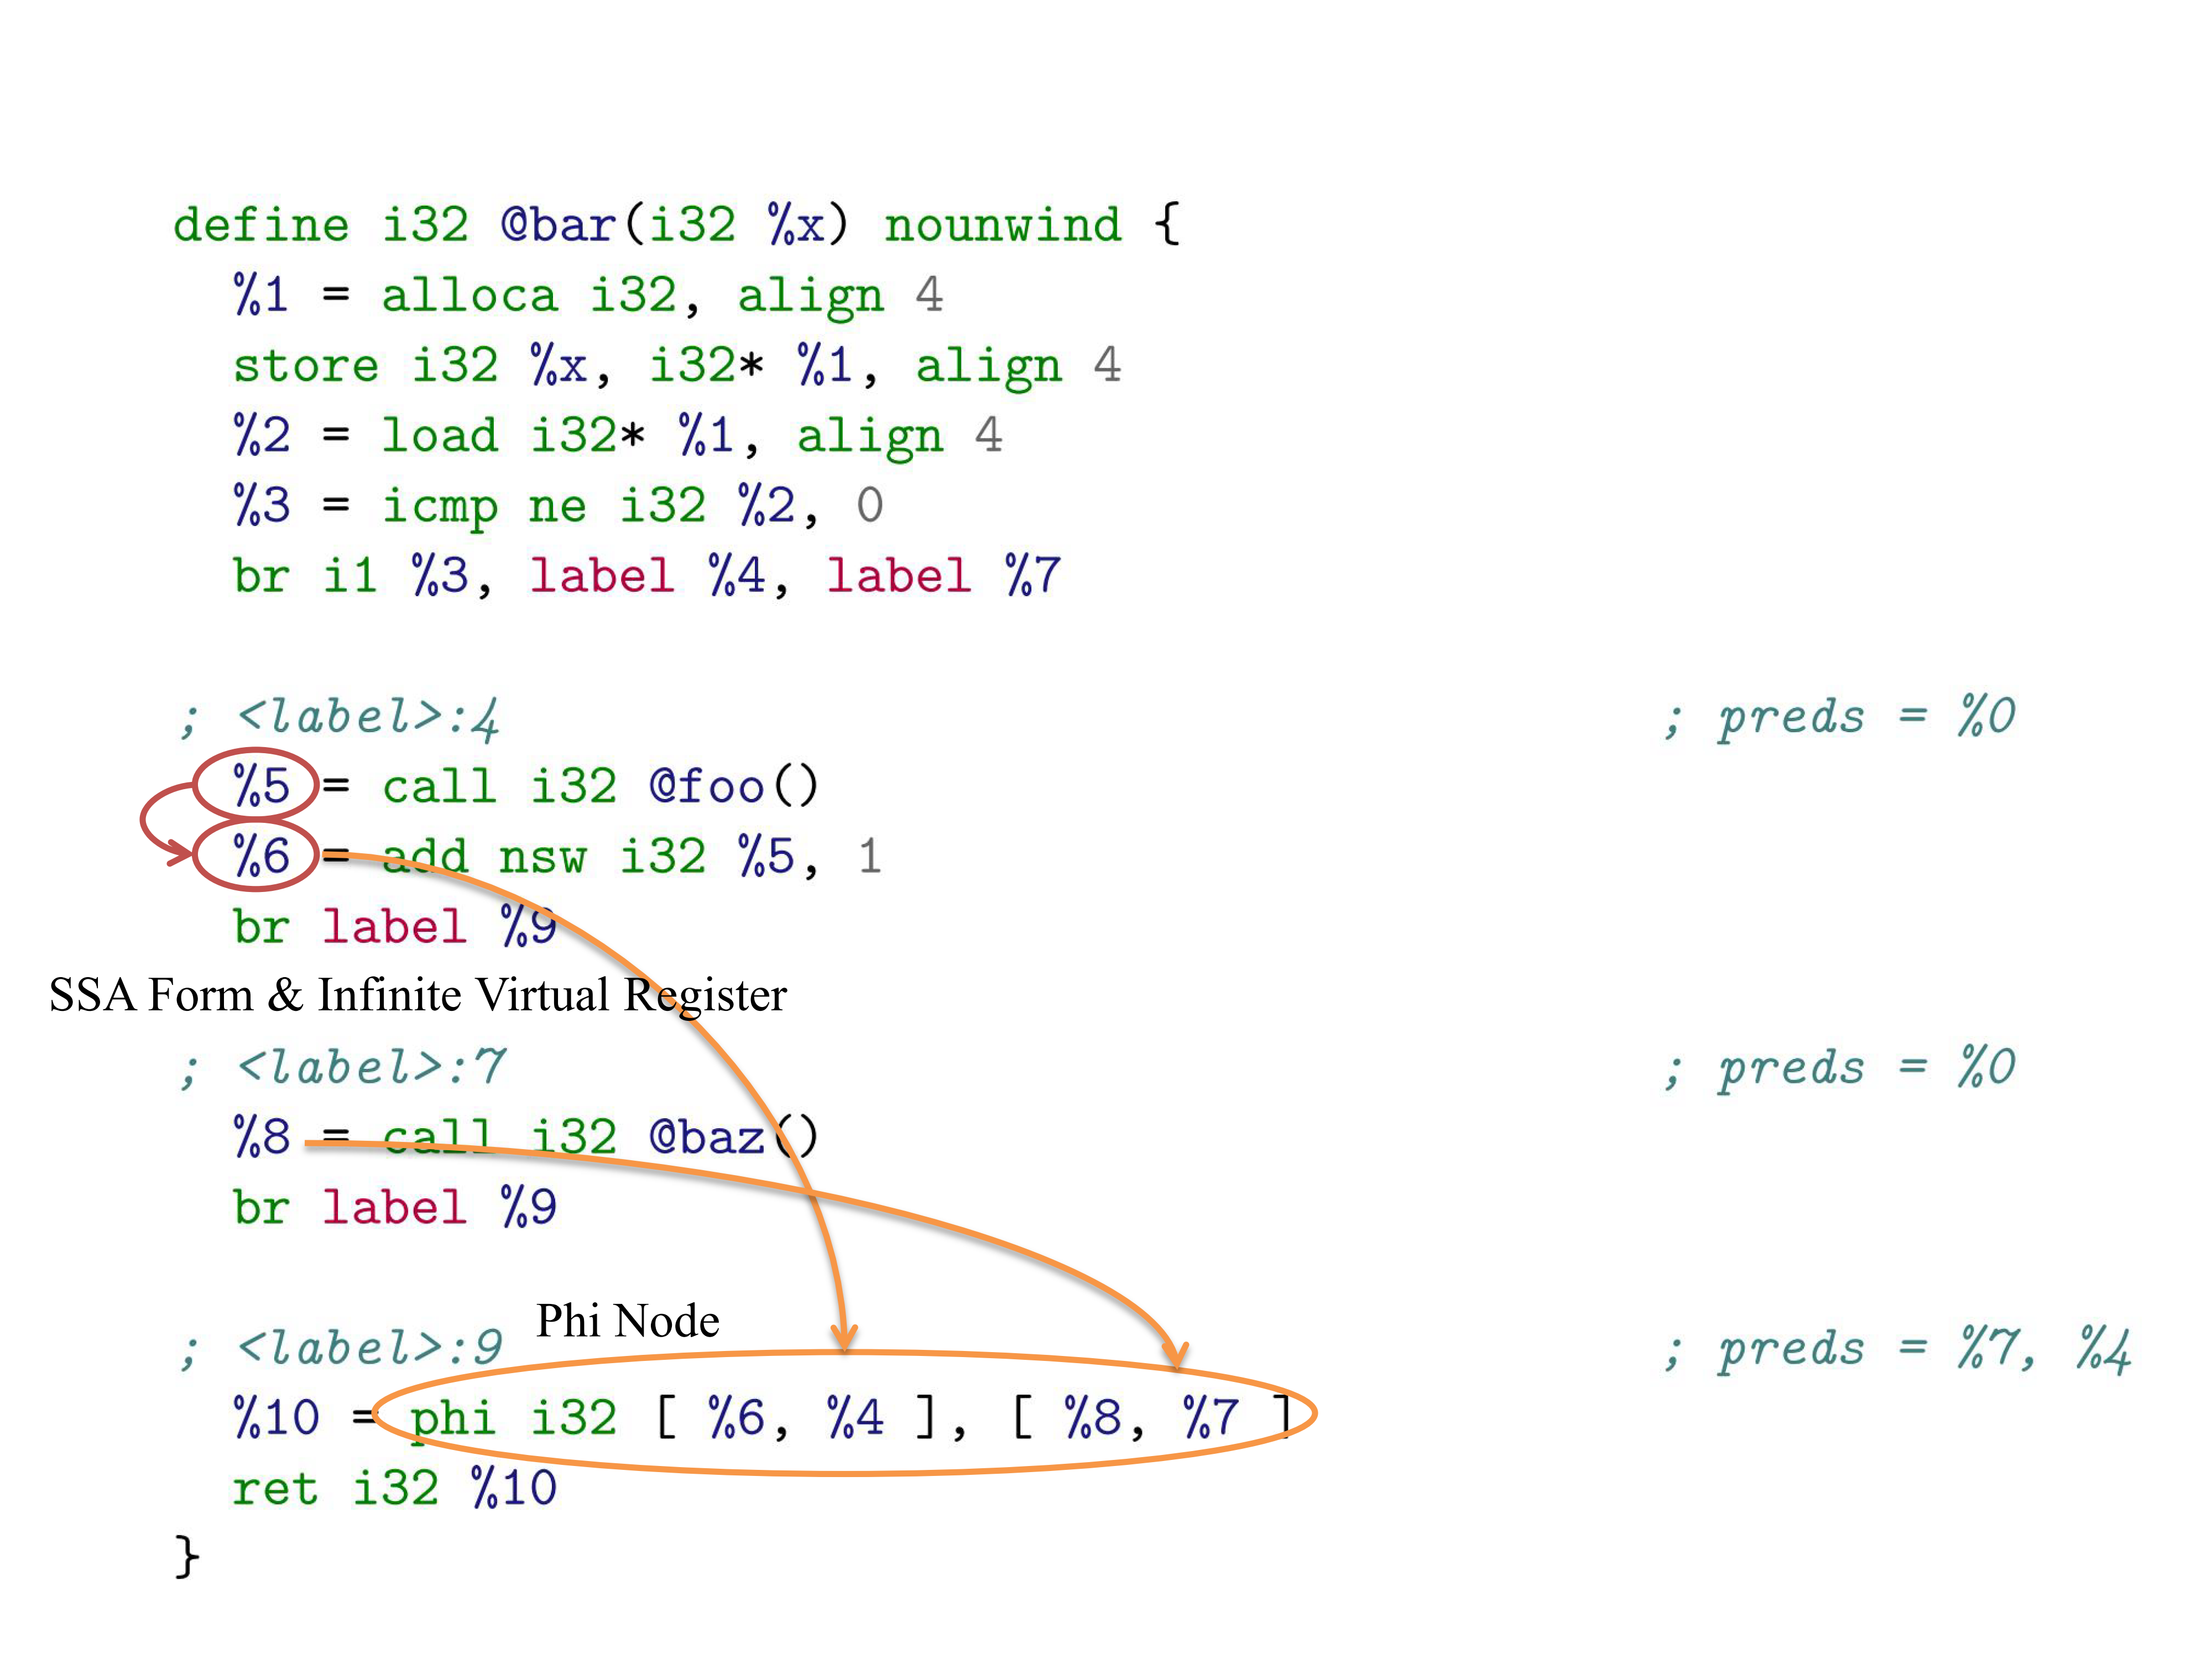
\includegraphics[scale=0.8]{fig/llvm_ir.png}
\end{figure}

\end{frame}

%----------- slide --------------------------------------------------%
\begin{frame}
  \frametitle{IR Builder 1/3}

LLVM IRBuilder is a class template that can be used as a convenient way
to create LLVM instructions. 

\begin{itemize}
  \item Module: The top level container of all other LLVM IR. It can contains
  global variables, functions, etc...
  \item Function: A function consists of a list of basic blocks and a list of arguments.
  \item Basic block: A container of instructions that can be executed sequentially.
  \item LLVMContext: A container of \textit{global} state in LLVM.
\end{itemize}

%MachineInstr (MI) also has builder, BuildMI, too.

\end{frame}

%----------- slide --------------------------------------------------%
\begin{frame}[shrink=15]
  \frametitle{IR Builder 2/3}

%\begin{Verbatim}[commandchars=\\\{\}]
\PY{c}{; ModuleID = \PYZsq{}fib.c\PYZsq{}}

\PY{k}{define} \PY{k}{i32} \PY{n+nv+vg}{@fib}\PY{p}{(}\PY{k}{i32} \PY{n+nv}{\PYZpc{}x}\PY{p}{)} \PY{k}{nounwind} \PY{k}{uwtable} \PY{p}{\PYZob{}}
\PY{n+nl}{entry:}
            \PY{p}{.}\PY{p}{.}\PY{p}{.}
  \PY{n+nv}{\PYZpc{}cmp} \PY{p}{=} \PY{k}{icmp} \PY{k}{sle} \PY{k}{i32} \PY{n+nv+nvAnonymous}{\PYZpc{}0}\PY{p}{,} \PY{l+m}{2}
  \PY{k}{br} \PY{k}{i1} \PY{n+nv}{\PYZpc{}cmp}\PY{p}{,} \PY{k+kt}{label} \PY{n+nv}{\PYZpc{}if.then}\PY{p}{,} \PY{k+kt}{label} \PY{n+nv}{\PYZpc{}if.else}

\PY{n+nl}{if.then:}                    \PY{c}{; preds = \PYZpc{}entry}
  \PY{k}{store} \PY{k}{i32} \PY{l+m}{1}\PY{p}{,} \PY{k}{i32}\PY{p}{*} \PY{n+nv}{\PYZpc{}sum}\PY{p}{,} \PY{k}{align} \PY{l+m}{4}
  \PY{k}{br} \PY{k+kt}{label} \PY{n+nv}{\PYZpc{}if.end}

\PY{n+nl}{if.else:}                    \PY{c}{; preds = \PYZpc{}entry}
            \PY{p}{.}\PY{p}{.}\PY{p}{.}
  \PY{n+nv}{\PYZpc{}call2} \PY{p}{=} \PY{k}{call} \PY{k}{i32} \PY{n+nv+vg}{@fib}\PY{p}{(}\PY{k}{i32} \PY{n+nv}{\PYZpc{}sub1}\PY{p}{)}
  \PY{n+nv}{\PYZpc{}add} \PY{p}{=} \PY{k}{add} \PY{k}{nsw} \PY{k}{i32} \PY{n+nv}{\PYZpc{}call}\PY{p}{,} \PY{n+nv}{\PYZpc{}call2}
  \PY{k}{store} \PY{k}{i32} \PY{n+nv}{\PYZpc{}add}\PY{p}{,} \PY{k}{i32}\PY{p}{*} \PY{n+nv}{\PYZpc{}sum}\PY{p}{,} \PY{k}{align} \PY{l+m}{4}
  \PY{k}{br} \PY{k+kt}{label} \PY{n+nv}{\PYZpc{}if.end}

\PY{n+nl}{if.end:}                     \PY{c}{; preds = \PYZpc{}if.else, \PYZpc{}if.then}
  \PY{n+nv+nvAnonymous}{\PYZpc{}3} \PY{p}{=} \PY{k}{load} \PY{k}{i32}\PY{p}{*} \PY{n+nv}{\PYZpc{}sum}\PY{p}{,} \PY{k}{align} \PY{l+m}{4}
  \PY{k}{ret} \PY{k}{i32} \PY{n+nv+nvAnonymous}{\PYZpc{}3}
\PY{p}{\PYZcb{}}
\end{Verbatim}


\begin{figure}
  \centering 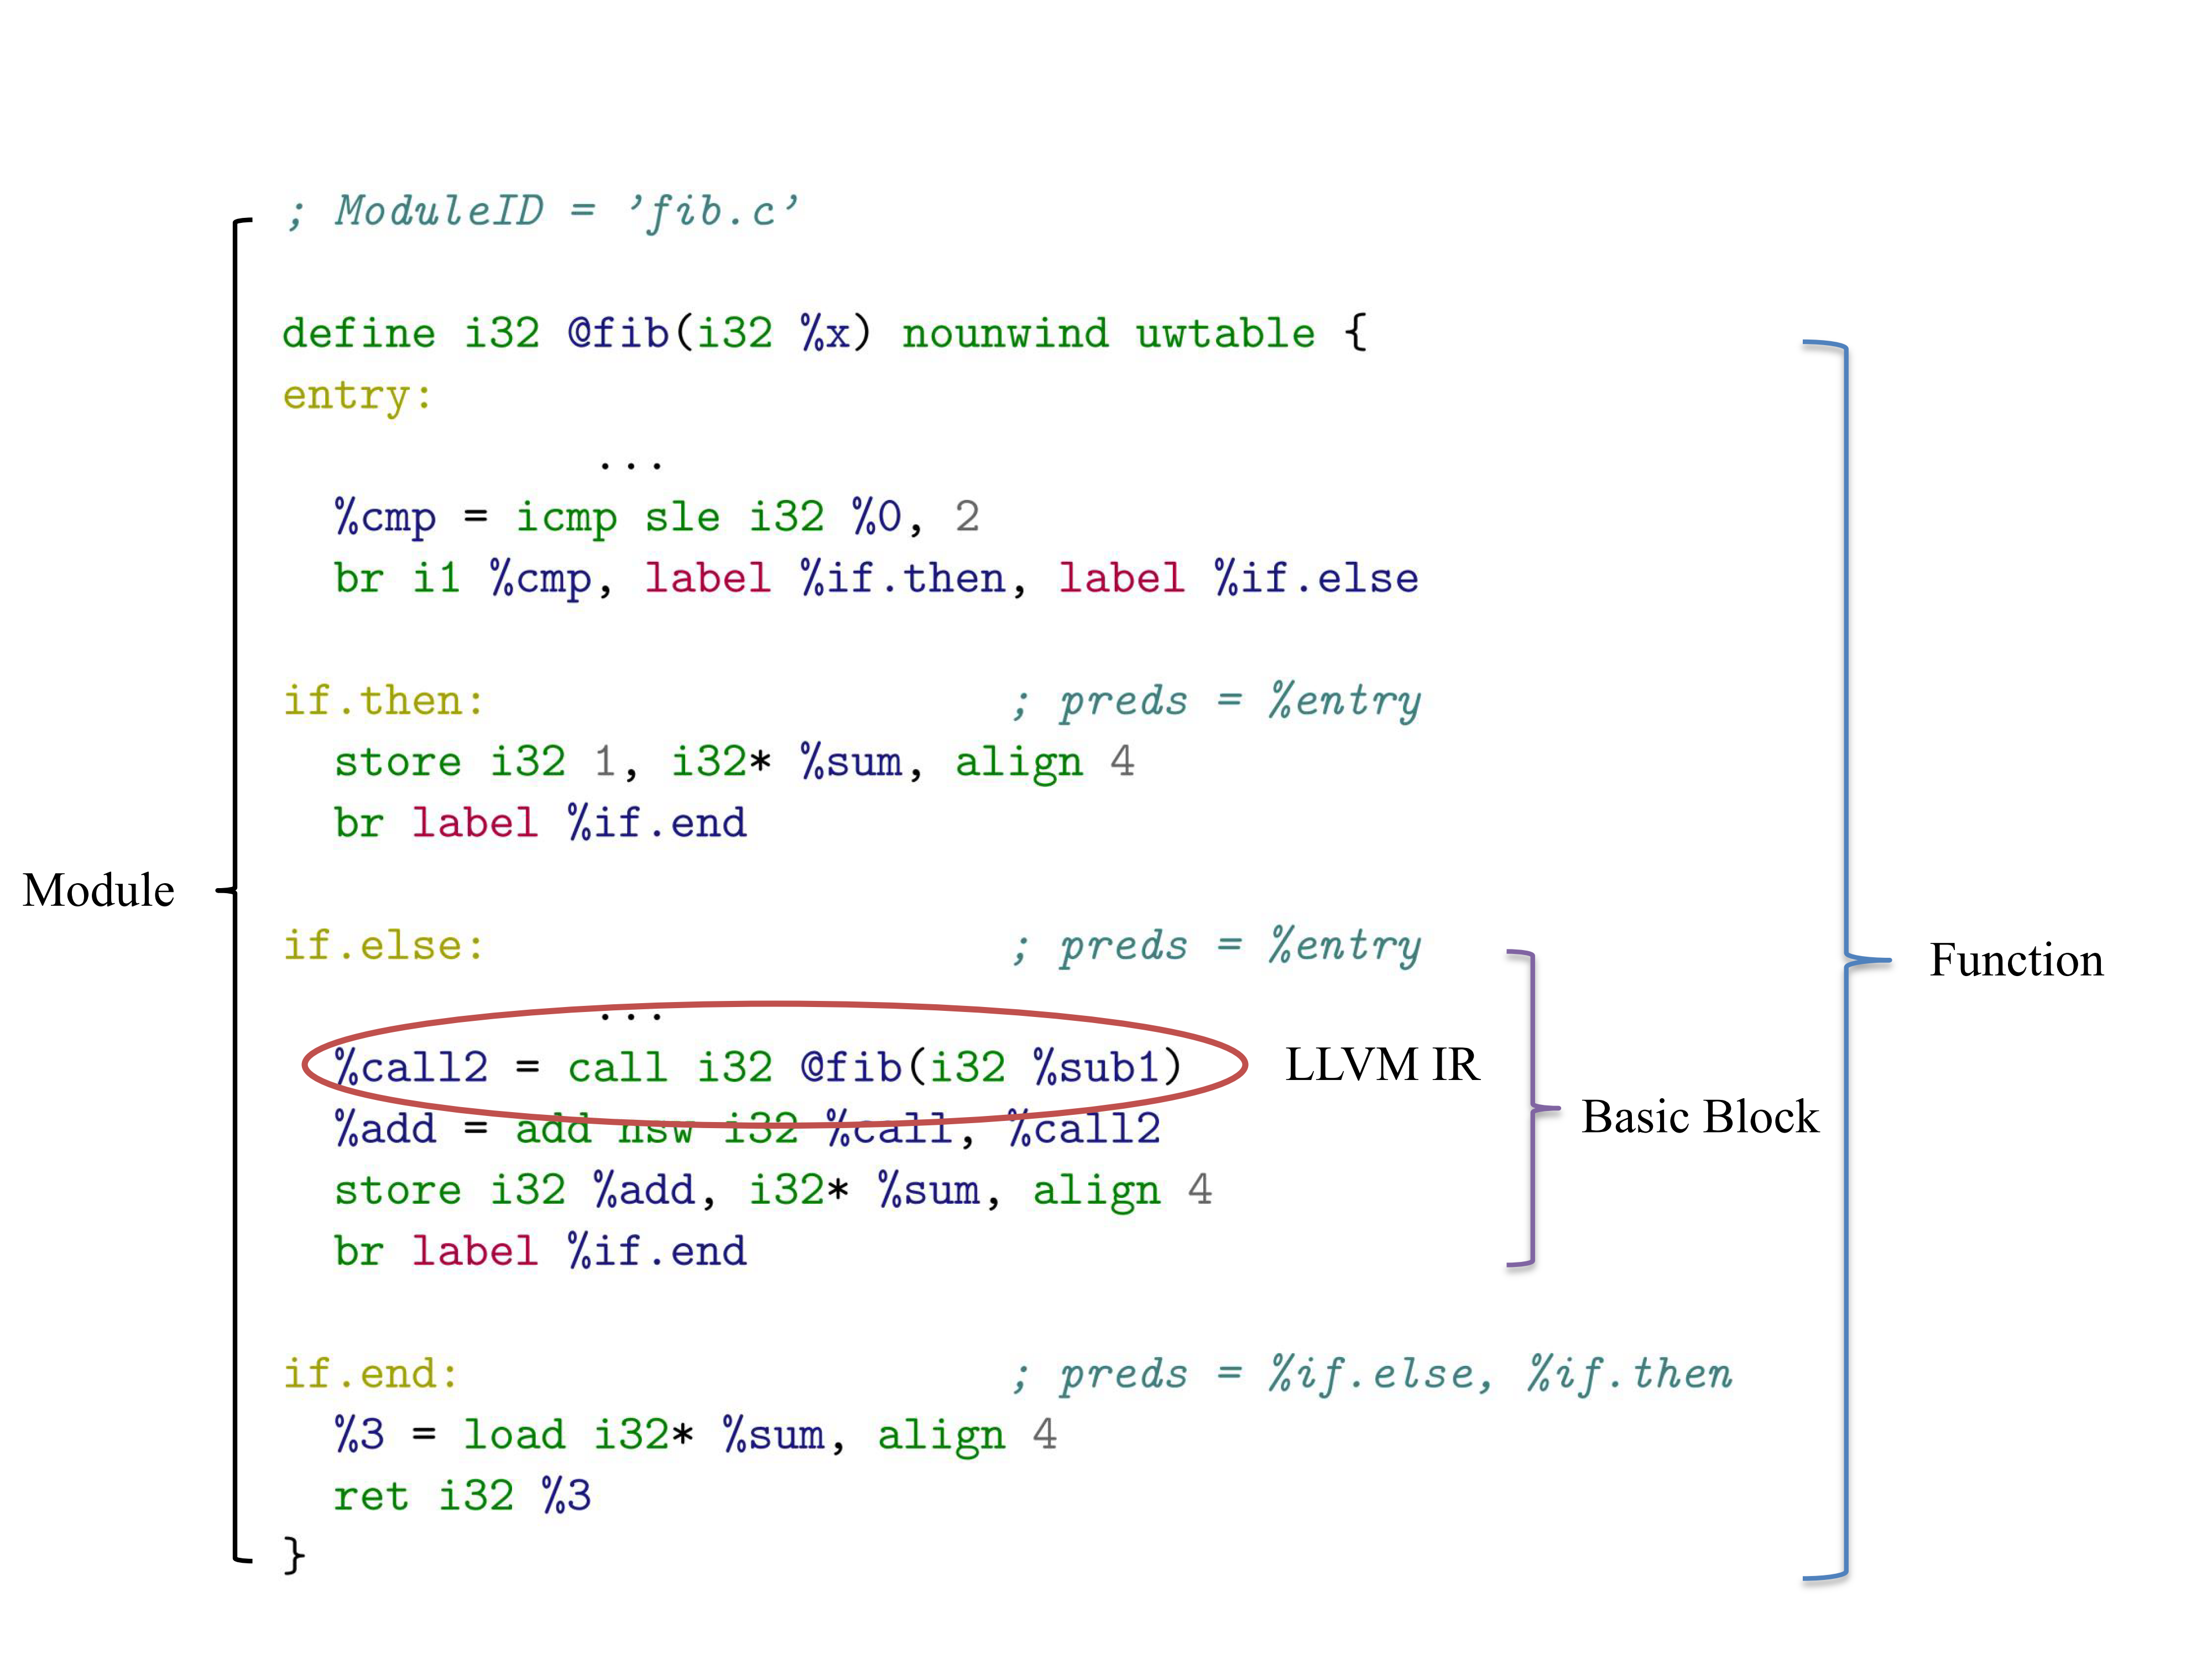
\includegraphics{fig/ir_builder.png}
\end{figure}

\end{frame}

%----------- slide --------------------------------------------------%
\begin{frame}[shrink=20]
  \frametitle{IR Builder 3/3}

\begin{Verbatim}[commandchars=\\\{\}]
\PY{c+c1}{// Create LLVMContext for latter use.}
\PY{n}{LLVMContext} \PY{n}{Context}\PY{p}{;}

\PY{c+c1}{// Create some module to put our function into it.}
\PY{n}{Module} \PY{o}{*}\PY{n}{M} \PY{o}{=} \PY{k}{new} \PY{n}{Module}\PY{p}{(}\PY{l+s}{\PYZdq{}}\PY{l+s}{test}\PY{l+s}{\PYZdq{}}\PY{p}{,} \PY{n}{Context}\PY{p}{)}\PY{p}{;}

\PY{c+c1}{// Create function inside the module}
\PY{n}{Function} \PY{o}{*}\PY{n}{Add1F} \PY{o}{=}
  \PY{n}{cast}\PY{o}{\PYZlt{}}\PY{n}{Function}\PY{o}{\PYZgt{}}\PY{p}{(}\PY{n}{M}\PY{o}{\PYZhy{}}\PY{o}{\PYZgt{}}\PY{n}{getOrInsertFunction}\PY{p}{(}\PY{l+s}{\PYZdq{}}\PY{l+s}{add1}\PY{l+s}{\PYZdq{}}\PY{p}{,} \PY{n}{Type}\PY{o}{:}\PY{o}{:}\PY{n}{getInt32Ty}\PY{p}{(}\PY{n}{Context}\PY{p}{)}\PY{p}{,}
                                        \PY{n}{Type}\PY{o}{:}\PY{o}{:}\PY{n}{getInt32Ty}\PY{p}{(}\PY{n}{Context}\PY{p}{)}\PY{p}{,}
                                        \PY{p}{(}\PY{n}{Type} \PY{o}{*}\PY{p}{)}\PY{l+m+mi}{0}\PY{p}{)}\PY{p}{)}\PY{p}{;}

\PY{c+c1}{// Add a basic block to the function.}
\PY{n}{BasicBlock} \PY{o}{*}\PY{n}{BB} \PY{o}{=} \PY{n}{BasicBlock}\PY{o}{:}\PY{o}{:}\PY{n}{Create}\PY{p}{(}\PY{n}{Context}\PY{p}{,} \PY{l+s}{\PYZdq{}}\PY{l+s}{EntryBlock}\PY{l+s}{\PYZdq{}}\PY{p}{,} \PY{n}{Add1F}\PY{p}{)}\PY{p}{;}

\PY{c+c1}{// Create a basic block builder. The builder will append instructions}
\PY{c+c1}{// to the basic block \PYZsq{}BB\PYZsq{}.}
\PY{n}{IRBuilder}\PY{o}{\PYZlt{}}\PY{o}{\PYZgt{}} \PY{n}{builder}\PY{p}{(}\PY{n}{BB}\PY{p}{)}\PY{p}{;}

\PY{c+c1}{// ... prepare operands for Add instrcution. ...}

\PY{c+c1}{// Create the add instruction, inserting it into the end of BB.}
\PY{n}{Value} \PY{o}{*}\PY{n}{Add} \PY{o}{=} \PY{n}{builder}\PY{p}{.}\PY{n}{CreateAdd}\PY{p}{(}\PY{n}{One}\PY{p}{,} \PY{n}{ArgX}\PY{p}{)}\PY{p}{;}
\end{Verbatim}


\end{frame}

%----------- slide --------------------------------------------------%
\begin{frame}

  \centering Let's start with a simple HelloWorld!

  \vspace\baselineskip

  \centering We will stick with LLVM 3.2 Release!

\end{frame}

%----------- slide --------------------------------------------------%
\begin{frame}[shrink=10]
  \frametitle{Step 1. Create Module}

  \vspace\baselineskip

\begin{Verbatim}[commandchars=\\\{\}]
\PY{c+cp}{\PYZsh{}}\PY{c+cp}{include \PYZdq{}llvm}\PY{c+cp}{/}\PY{c+cp}{LLVMContext.h\PYZdq{}}
\PY{c+cp}{\PYZsh{}}\PY{c+cp}{include \PYZdq{}llvm}\PY{c+cp}{/}\PY{c+cp}{Module.h\PYZdq{}}
\PY{c+cp}{\PYZsh{}}\PY{c+cp}{include \PYZdq{}llvm}\PY{c+cp}{/}\PY{c+cp}{IRBuilder.h\PYZdq{}}

\PY{k+kt}{int} \PY{n+nf}{main}\PY{p}{(}\PY{p}{)}
\PY{p}{\PYZob{}}
  \PY{n}{llvm}\PY{o}{:}\PY{o}{:}\PY{n}{LLVMContext}\PY{o}{\PYZam{}} \PY{n}{context} \PY{o}{=} \PY{n}{llvm}\PY{o}{:}\PY{o}{:}\PY{n}{getGlobalContext}\PY{p}{(}\PY{p}{)}\PY{p}{;}
  \PY{n}{llvm}\PY{o}{:}\PY{o}{:}\PY{n}{Module}\PY{o}{*} \PY{n}{module} \PY{o}{=} \PY{k}{new} \PY{n}{llvm}\PY{o}{:}\PY{o}{:}\PY{n}{Module}\PY{p}{(}\PY{l+s}{\PYZdq{}}\PY{l+s}{top}\PY{l+s}{\PYZdq{}}\PY{p}{,} \PY{n}{context}\PY{p}{)}\PY{p}{;}
  \PY{n}{llvm}\PY{o}{:}\PY{o}{:}\PY{n}{IRBuilder}\PY{o}{\PYZlt{}}\PY{o}{\PYZgt{}} \PY{n}{builder}\PY{p}{(}\PY{n}{context}\PY{p}{)}\PY{p}{;} 

  \PY{n}{module}\PY{o}{\PYZhy{}}\PY{o}{\PYZgt{}}\PY{n}{dump}\PY{p}{(} \PY{p}{)}\PY{p}{;}
\PY{p}{\PYZcb{}}
\end{Verbatim}


  \vspace\baselineskip

\begin{Verbatim}[commandchars=\\\{\}]
\PY{c}{; ModuleID = \PYZsq{}top\PYZsq{}}
\end{Verbatim}


\end{frame}

%----------- slide --------------------------------------------------%
\begin{frame}[shrink=15]
  \frametitle{Step 2. Create Function}

  \vspace\baselineskip

\begin{Verbatim}[commandchars=\\\{\}]
          \PY{p}{.}\PY{p}{.}\PY{p}{.}

  \PY{n}{llvm}\PY{o}{:}\PY{o}{:}\PY{n}{FunctionType} \PY{o}{*}\PY{n}{funcType} \PY{o}{=} 
      \PY{n}{llvm}\PY{o}{:}\PY{o}{:}\PY{n}{FunctionType}\PY{o}{:}\PY{o}{:}\PY{n}{get}\PY{p}{(}\PY{n}{builder}\PY{p}{.}\PY{n}{getInt32Ty}\PY{p}{(}\PY{p}{)}\PY{p}{,} \PY{n+nb}{false}\PY{p}{)}\PY{p}{;}
  \PY{n}{llvm}\PY{o}{:}\PY{o}{:}\PY{n}{Function} \PY{o}{*}\PY{n}{mainFunc} \PY{o}{=} 
      \PY{n}{llvm}\PY{o}{:}\PY{o}{:}\PY{n}{Function}\PY{o}{:}\PY{o}{:}\PY{n}{Create}\PY{p}{(}\PY{n}{funcType}\PY{p}{,}
                             \PY{n}{llvm}\PY{o}{:}\PY{o}{:}\PY{n}{Function}\PY{o}{:}\PY{o}{:}\PY{n}{ExternalLinkage}\PY{p}{,}
                             \PY{l+s}{\PYZdq{}}\PY{l+s}{main}\PY{l+s}{\PYZdq{}}\PY{p}{,} \PY{n}{module}\PY{p}{)}\PY{p}{;}

  \PY{n}{module}\PY{o}{\PYZhy{}}\PY{o}{\PYZgt{}}\PY{n}{dump}\PY{p}{(} \PY{p}{)}\PY{p}{;}
\PY{p}{\PYZcb{}}
\end{Verbatim}


  \vspace\baselineskip

\begin{Verbatim}[commandchars=\\\{\}]
\PY{c}{; ModuleID = \PYZsq{}top\PYZsq{}}

\PY{k}{declare} \PY{k}{i32} \PY{n+nv+vg}{@main}\PY{p}{(}\PY{p}{)}
\end{Verbatim}


\end{frame}

%----------- slide --------------------------------------------------%
\begin{frame}[shrink=15]
  \frametitle{Step 3. Create Basic Block}

  \vspace\baselineskip

\begin{Verbatim}[commandchars=\\\{\}]
          \PY{p}{.}\PY{p}{.}\PY{p}{.}

  \PY{n}{llvm}\PY{o}{:}\PY{o}{:}\PY{n}{BasicBlock} \PY{o}{*}\PY{n}{entry} \PY{o}{=}
      \PY{n}{llvm}\PY{o}{:}\PY{o}{:}\PY{n}{BasicBlock}\PY{o}{:}\PY{o}{:}\PY{n}{Create}\PY{p}{(}\PY{n}{context}\PY{p}{,} \PY{l+s}{\PYZdq{}}\PY{l+s}{entrypoint}\PY{l+s}{\PYZdq{}}\PY{p}{,} \PY{n}{mainFunc}\PY{p}{)}\PY{p}{;}
  \PY{n}{builder}\PY{p}{.}\PY{n}{SetInsertPoint}\PY{p}{(}\PY{n}{entry}\PY{p}{)}\PY{p}{;}

  \PY{n}{module}\PY{o}{\PYZhy{}}\PY{o}{\PYZgt{}}\PY{n}{dump}\PY{p}{(} \PY{p}{)}\PY{p}{;}
\PY{p}{\PYZcb{}}
\end{Verbatim}


  \vspace\baselineskip

\begin{Verbatim}[commandchars=\\\{\}]
\PY{c}{; ModuleID = \PYZsq{}top\PYZsq{}}

\PY{k}{define} \PY{k}{i32} \PY{n+nv+vg}{@main}\PY{p}{(}\PY{p}{)} \PY{p}{\PYZob{}}
\PY{n+nl}{entrypoint:}
\PY{p}{\PYZcb{}}
\end{Verbatim}


\end{frame}

%----------- slide --------------------------------------------------%
\begin{frame}[shrink=15]
  \frametitle{Step 4. Add "hello world" into the Module}

  \vspace\baselineskip

\begin{Verbatim}[commandchars=\\\{\}]
          \PY{p}{.}\PY{p}{.}\PY{p}{.}

  \PY{n}{llvm}\PY{o}{:}\PY{o}{:}\PY{n}{Value} \PY{o}{*}\PY{n}{helloWorld}
      \PY{o}{=} \PY{n}{builder}\PY{p}{.}\PY{n}{CreateGlobalStringPtr}\PY{p}{(}\PY{l+s}{\PYZdq{}}\PY{l+s}{hello world!}\PY{l+s+se}{\PYZbs{}n}\PY{l+s}{\PYZdq{}}\PY{p}{)}\PY{p}{;}

  \PY{n}{module}\PY{o}{\PYZhy{}}\PY{o}{\PYZgt{}}\PY{n}{dump}\PY{p}{(} \PY{p}{)}\PY{p}{;}
\PY{p}{\PYZcb{}}
\end{Verbatim}


  \vspace\baselineskip

\begin{Verbatim}[commandchars=\\\{\}]
\PY{c}{; ModuleID = \PYZsq{}top\PYZsq{}}

\PY{n+nv+vg}{@0} \PY{p}{=} \PY{k}{private} \PY{k}{unnamed_addr} \PY{k}{constant} \PY{p}{[}\PY{l+m}{14} \PY{k}{x} \PY{k}{i8}\PY{p}{]} \PY{k}{c}\PY{l+s}{\PYZdq{}hello world!\PYZbs{}0A\PYZbs{}00\PYZdq{}}

\PY{k}{define} \PY{k+kt}{void} \PY{n+nv+vg}{@main}\PY{p}{(}\PY{p}{)} \PY{p}{\PYZob{}}
\PY{n+nl}{entrypoint:}
\PY{p}{\PYZcb{}}
\end{Verbatim}


\end{frame}

%----------- slide --------------------------------------------------%
\begin{frame}[shrink=15]
  \frametitle{Step 5. Declare "puts" method}

  \vspace\baselineskip

\begin{Verbatim}[commandchars=\\\{\}]
          \PY{p}{.}\PY{p}{.}\PY{p}{.}

  \PY{n}{std}\PY{o}{:}\PY{o}{:}\PY{n}{vector}\PY{o}{\PYZlt{}}\PY{n}{llvm}\PY{o}{:}\PY{o}{:}\PY{n}{Type} \PY{o}{*}\PY{o}{\PYZgt{}} \PY{n}{putsArgs}\PY{p}{;}
  \PY{n}{putsArgs}\PY{p}{.}\PY{n}{push\PYZus{}back}\PY{p}{(}\PY{n}{builder}\PY{p}{.}\PY{n}{getInt8Ty}\PY{p}{(}\PY{p}{)}\PY{o}{\PYZhy{}}\PY{o}{\PYZgt{}}\PY{n}{getPointerTo}\PY{p}{(}\PY{p}{)}\PY{p}{)}\PY{p}{;}
  \PY{n}{llvm}\PY{o}{:}\PY{o}{:}\PY{n}{ArrayRef}\PY{o}{\PYZlt{}}\PY{n}{llvm}\PY{o}{:}\PY{o}{:}\PY{n}{Type}\PY{o}{*}\PY{o}{\PYZgt{}}  \PY{n}{argsRef}\PY{p}{(}\PY{n}{putsArgs}\PY{p}{)}\PY{p}{;}

  \PY{n}{llvm}\PY{o}{:}\PY{o}{:}\PY{n}{FunctionType} \PY{o}{*}\PY{n}{putsType} \PY{o}{=} 
    \PY{n}{llvm}\PY{o}{:}\PY{o}{:}\PY{n}{FunctionType}\PY{o}{:}\PY{o}{:}\PY{n}{get}\PY{p}{(}\PY{n}{builder}\PY{p}{.}\PY{n}{getInt32Ty}\PY{p}{(}\PY{p}{)}\PY{p}{,} \PY{n}{argsRef}\PY{p}{,} \PY{n+nb}{false}\PY{p}{)}\PY{p}{;}
  \PY{n}{llvm}\PY{o}{:}\PY{o}{:}\PY{n}{Constant} \PY{o}{*}\PY{n}{putsFunc}
    \PY{o}{=} \PY{n}{module}\PY{o}{\PYZhy{}}\PY{o}{\PYZgt{}}\PY{n}{getOrInsertFunction}\PY{p}{(}\PY{l+s}{\PYZdq{}}\PY{l+s}{puts}\PY{l+s}{\PYZdq{}}\PY{p}{,} \PY{n}{putsType}\PY{p}{)}\PY{p}{;}

  \PY{n}{module}\PY{o}{\PYZhy{}}\PY{o}{\PYZgt{}}\PY{n}{dump}\PY{p}{(}\PY{p}{)}\PY{p}{;}
\PY{p}{\PYZcb{}}
\end{Verbatim}


  \vspace\baselineskip

\begin{Verbatim}[commandchars=\\\{\}]
\PY{c}{; ModuleID = \PYZsq{}top\PYZsq{}}

\PY{n+nv+vg}{@0} \PY{p}{=} \PY{k}{private} \PY{err}{u}\PY{err}{n}\PY{err}{n}\PY{err}{a}\PY{err}{m}\PY{err}{e}\PY{err}{d}\PY{err}{\PYZus{}}\PY{err}{a}\PY{err}{d}\PY{err}{d}\PY{err}{r} \PY{k}{constant} \PY{p}{[}\PY{l+m}{14} \PY{k}{x} \PY{k}{i8}\PY{p}{]} \PY{k}{c}\PY{l+s}{\PYZdq{}hello world!\PYZbs{}0A\PYZbs{}00\PYZdq{}}

\PY{k}{define} \PY{k+kt}{void} \PY{n+nv+vg}{@main}\PY{p}{(}\PY{p}{)} \PY{p}{\PYZob{}}
\PY{n+nl}{entrypoint:}
\PY{p}{\PYZcb{}}

\PY{k}{declare} \PY{k}{i32} \PY{n+nv+vg}{@puts}\PY{p}{(}\PY{k}{i8}\PY{p}{*}\PY{p}{)}
\end{Verbatim}


\end{frame}

%----------- slide --------------------------------------------------%
\begin{frame}[shrink=15]
  \frametitle{Step 6. Call "puts" with "hello world"}

  \vspace\baselineskip

\begin{Verbatim}[commandchars=\\\{\}]
          \PY{p}{.}\PY{p}{.}\PY{p}{.}

  \PY{n}{builder}\PY{p}{.}\PY{n}{CreateCall}\PY{p}{(}\PY{n}{putsFunc}\PY{p}{,} \PY{n}{helloWorld}\PY{p}{)}\PY{p}{;}
  \PY{n}{builder}\PY{p}{.}\PY{n}{CreateRetVoid}\PY{p}{(}\PY{p}{)}\PY{p}{;}

  \PY{n}{module}\PY{o}{\PYZhy{}}\PY{o}{\PYZgt{}}\PY{n}{dump}\PY{p}{(}\PY{p}{)}\PY{p}{;}
\PY{p}{\PYZcb{}}
\end{Verbatim}


  \vspace\baselineskip

\begin{Verbatim}[commandchars=\\\{\}]
\PY{c}{; ModuleID = \PYZsq{}top\PYZsq{}}

\PY{n+nv+vg}{@0} \PY{p}{=} \PY{k}{private} \PY{err}{u}\PY{err}{n}\PY{err}{n}\PY{err}{a}\PY{err}{m}\PY{err}{e}\PY{err}{d}\PY{err}{\PYZus{}}\PY{err}{a}\PY{err}{d}\PY{err}{d}\PY{err}{r} \PY{k}{constant} \PY{p}{[}\PY{l+m}{14} \PY{k}{x} \PY{k}{i8}\PY{p}{]} \PY{k}{c}\PY{l+s}{\PYZdq{}hello world!\PYZbs{}0A\PYZbs{}00\PYZdq{}}

\PY{k}{define} \PY{k+kt}{void} \PY{n+nv+vg}{@main}\PY{p}{(}\PY{p}{)} \PY{p}{\PYZob{}}
\PY{n+nl}{entrypoint:}
  \PY{n+nv+nvAnonymous}{\PYZpc{}0} \PY{p}{=} \PY{k}{call} \PY{k}{i32} \PY{n+nv+vg}{@puts}\PY{p}{(}\PY{k}{i8}\PY{p}{*} \PY{k}{getelementptr} \PY{k}{inbounds} \PY{p}{(}\PY{p}{[}\PY{l+m}{14} \PY{k}{x} \PY{k}{i8}\PY{p}{]}\PY{p}{*} \PY{n+nv+vg}{@0}\PY{p}{,} \PY{k}{i32} \PY{l+m}{0}\PY{p}{,} \PY{k}{i32} \PY{l+m}{0}\PY{p}{)}\PY{p}{)}
  \PY{k}{ret} \PY{k+kt}{void}
\PY{p}{\PYZcb{}}

\PY{k}{declare} \PY{k}{i32} \PY{n+nv+vg}{@puts}\PY{p}{(}\PY{k}{i8}\PY{p}{*}\PY{p}{)}
\end{Verbatim}


\end{frame}

%----------- slide --------------------------------------------------%
\begin{frame}
  \frametitle{Lowering Flow Overview}

\begin{figure}
  \centering 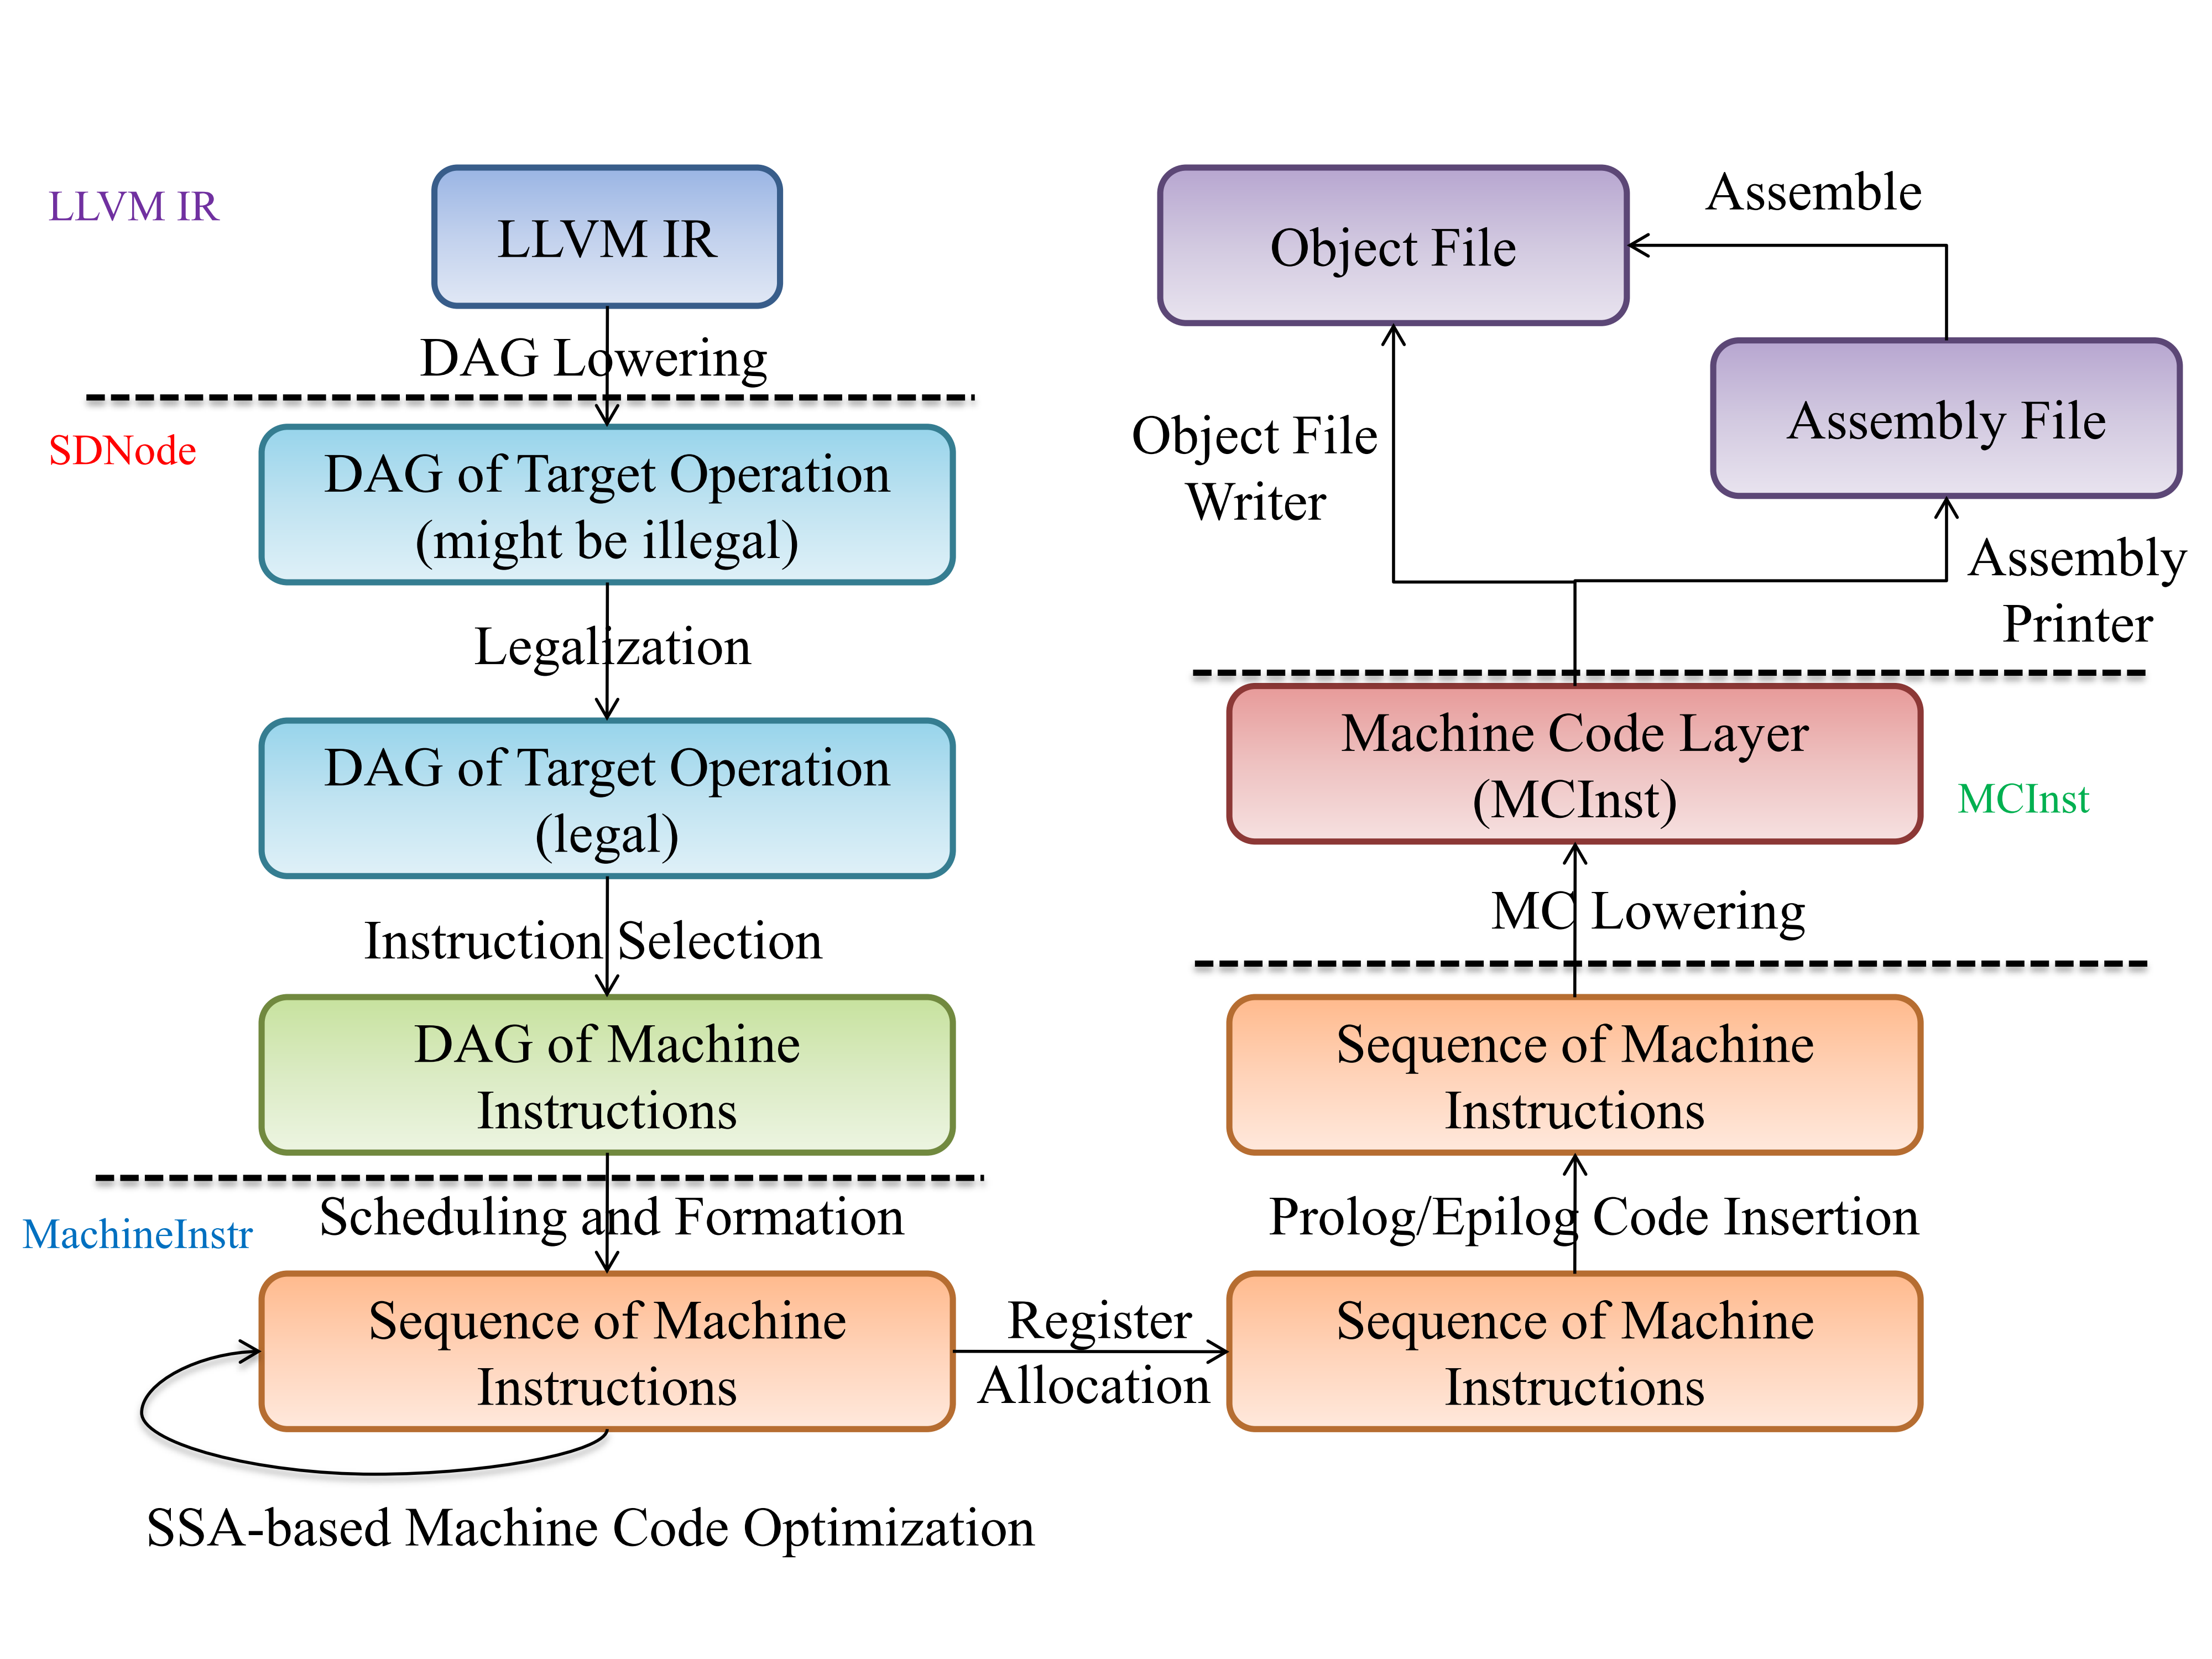
\includegraphics[scale=0.425]{fig/lowering_flow.png}
\end{figure}

\end{frame}

%----------- slide --------------------------------------------------%
\begin{frame}[fragile]
  \frametitle{LLVM \ensuremath{\rightarrow} DAG}

\begin{figure}
  \centering 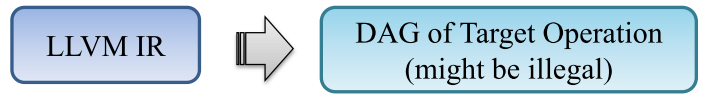
\includegraphics[scale=0.3]{fig/ir_to_dag.png}
\end{figure}

  We first translate a sequence of LLVM IR into a SelectionDAG to make
instruction selection easier. DAG also make optimization efficiently,
CSE (Common Subexpression Elimination), for example.

  \vspace\baselineskip

  For each use and def in the LLVM IR, an SDNode (SelectionDAG Node) is
created. The SDNode could be intrinsic SDNode or target defined SDNode.

  \vspace\baselineskip

\begin{Verbatim}[commandchars=\\\{\}]
\PY{n+nv}{\PYZdl{} }llc \PYZhy{}view\PYZhy{}dag\PYZhy{}combine1\PYZhy{}dags fib.ll
\PY{n+nv}{\PYZdl{} }dot \PYZhy{}Tpng dag.fib.dot \PYZhy{}o dag.fib.png
\end{Verbatim}

\end{frame}

%----------- slide --------------------------------------------------%
\begin{frame}
  \frametitle{LLVM \ensuremath{\rightarrow} DAG}

\begin{figure}
  \centering 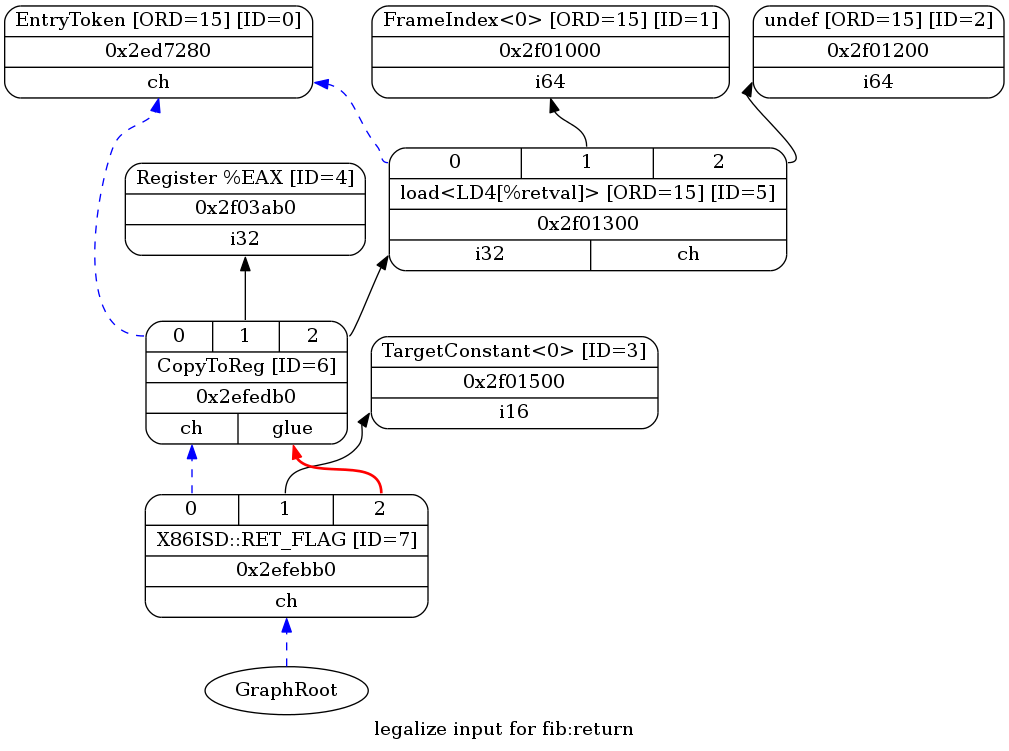
\includegraphics[scale=0.275]{dot/view-legalize-dags-fib.png}
\end{figure}

\end{frame}

%----------- slide --------------------------------------------------%
\begin{frame}[fragile]
  \frametitle{Legalize}

\begin{figure}
  \centering 
\includegraphics[scale=0.3]{fig/legalize.png}
\end{figure}

  Target machine might not support some of LLVM types or operations, we need to
\textcolor{red}{legalize} previous DAG.

\begin{Verbatim}[commandchars=\\\{\}]
\PY{n+nv}{\PYZdl{} }llc \PYZhy{}view\PYZhy{}dag\PYZhy{}combine2\PYZhy{}dags fib.ll
\end{Verbatim}
 
\end{frame}

%----------- slide --------------------------------------------------%
\begin{frame}[fragile]
  \frametitle{IR DAG \ensuremath{\rightarrow} Machine DAG}

\begin{figure}
  \centering 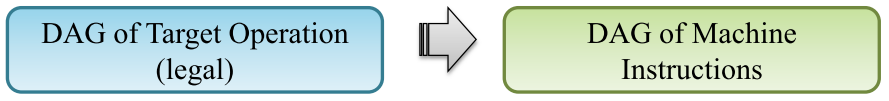
\includegraphics[scale=0.3]{fig/dag_to_dag.png}
\end{figure}

  The instruction selector match IR SDNode into MachineSDNode. MachineSDNode
represents everything that will be needed to construct a MachineInstr (MI).

  \vspace\baselineskip

\begin{Verbatim}[commandchars=\\\{\}]
\PY{c}{\PYZsh{} displays the DAG before instruction selection}
\PY{n+nv}{\PYZdl{} }llc \PYZhy{}view\PYZhy{}isel\PYZhy{}dags fib.ll
\PY{c}{\PYZsh{} displays the DAG before instruction scheduling}
\PY{n+nv}{\PYZdl{} }llc \PYZhy{}view\PYZhy{}sched\PYZhy{}dags fib.ll
\end{Verbatim}

\end{frame}


%----------- slide --------------------------------------------------%
\begin{frame}[fragile]
  \frametitle{Scheduling and Formation}

\begin{figure}
  \centering 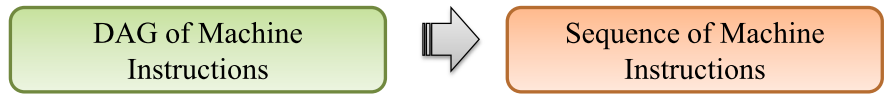
\includegraphics[scale=0.3]{fig/dag_to_mi.png}
\end{figure}

Machine DAG are deconstructed and their instruction are turned into
list of MachineInstr (MI). The scheduler has to decide in what order
the instructions (MI) are emitted.

  \vspace\baselineskip

\begin{Verbatim}[commandchars=\\\{\}]
\PY{n+nv}{\PYZdl{} }llc \PYZhy{}print\PYZhy{}machineinstrs fib.ll
\end{Verbatim}

  \vspace\baselineskip

\end{frame}

%----------- slide --------------------------------------------------%
\begin{frame}
  \frametitle{SSA-based Machine Code Optimization}

Ths list of MachineInstr is still in SSA form. We can perform target-specific
low-level optimization before doing register allocation. For example, LICM
(Loop Invariant Code Motion).

  \vspace\baselineskip

\begin{itemize}
  \item addMachineSSAOptimization (lib/CodeGen/Passes.cpp)
\end{itemize}

\end{frame}

%----------- slide --------------------------------------------------%
\begin{frame}
  \frametitle{Register Allocation}

All virtual registers are eliminated at this stage. The register allocator
assigns physical register to each virtual register if possible. After register
allocation, the list is not SSA form anymore.

\end{frame}

%----------- slide --------------------------------------------------%
\begin{frame}
  \frametitle{Prologue/Epilogue Code Insertion}

We insert prologue/epilogue code sequence into function beginning/end
respectively. All abstract stack frame references are turned into memory
address relative to the stack/frame pointer.

\end{frame}


%----------- slide --------------------------------------------------%
\begin{frame}
  \frametitle{What We Have Now?}

  C \ensuremath{\rightarrow} LLVM IR \ensuremath{\rightarrow} IR DAG
 \ensuremath{\rightarrow} Machine DAG \ensuremath{\rightarrow} MachineInstr (MI)
\end{frame}

%----------- slide --------------------------------------------------%
\begin{frame}
  \frametitle{Code Emission}

\begin{figure}
  \centering 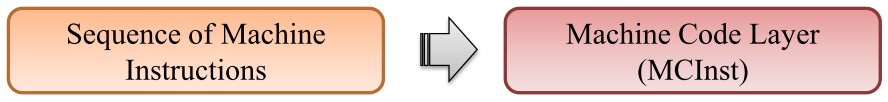
\includegraphics[scale=0.3]{fig/mi_to_mc.png}
\end{figure}

This stage lowers MachineInstr (MI) to MCInst (MC).

\begin{itemize}
  \item MachineInstr (MI): Abstraction of target instruction, consists of opcode and operand only. We have MachineFunction and MachineBasicBlock as containers for MI.
  \item MCInst (MC): Abstraction of object file. No function, global variable ...etc, but only label, directive and instruction.
\end{itemize}

\end{frame}

%----------- slide --------------------------------------------------%
\begin{frame}[fragile]
  \frametitle{Machine Code (MC) Layer}

  MC layer works at the level of abstraction of object file.

\begin{Verbatim}[commandchars=\\\{\}]
\PY{n+nv}{\PYZdl{} }llc \PYZhy{}show\PYZhy{}mc\PYZhy{}inst fib.ll
\PY{n+nv}{\PYZdl{} }llc \PYZhy{}show\PYZhy{}mc\PYZhy{}encoding fib.ll
\end{Verbatim}

\end{frame}

%----------- slide --------------------------------------------------%
%\begin{frame}
%  \frametitle{MC Layer Overview}
%
%\begin{figure}
%  \centering 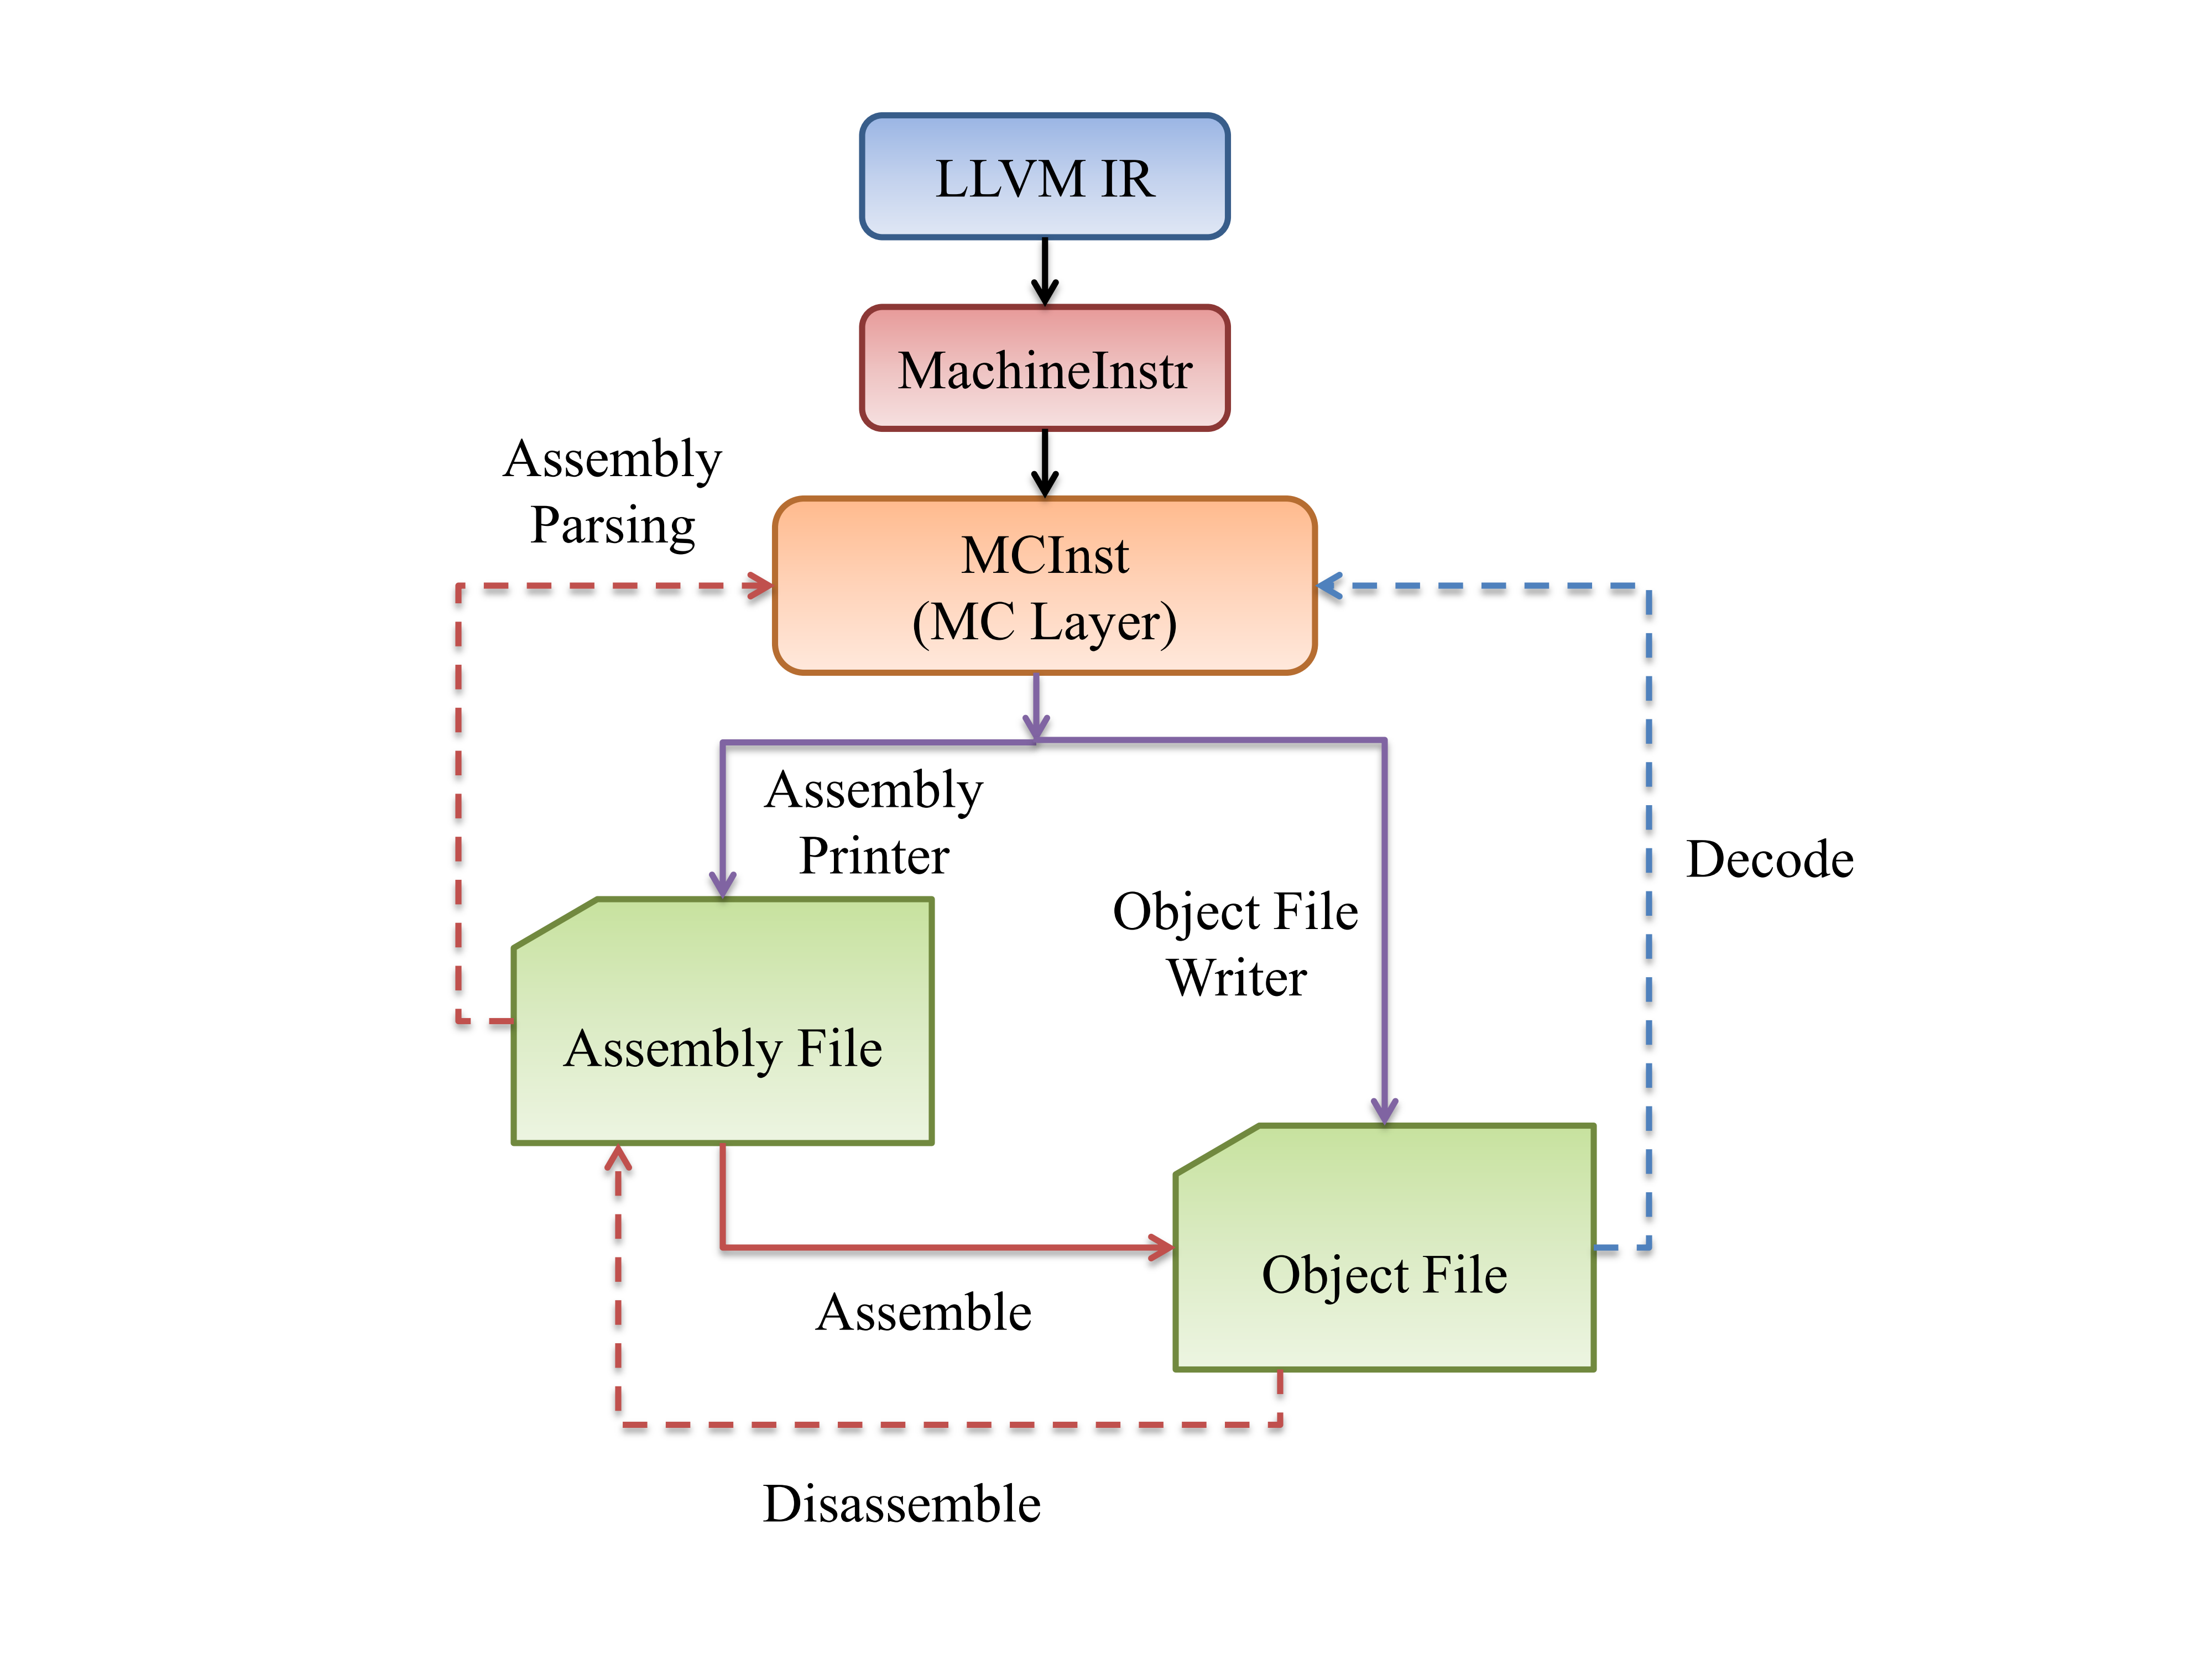
\includegraphics[scale=0.425]{fig/mc_layer_overview.png}
%\end{figure}
%
%\end{frame}

%----------- slide --------------------------------------------------%
\begin{frame}
  \frametitle{MC Layer Flow}

\begin{figure}
  \centering 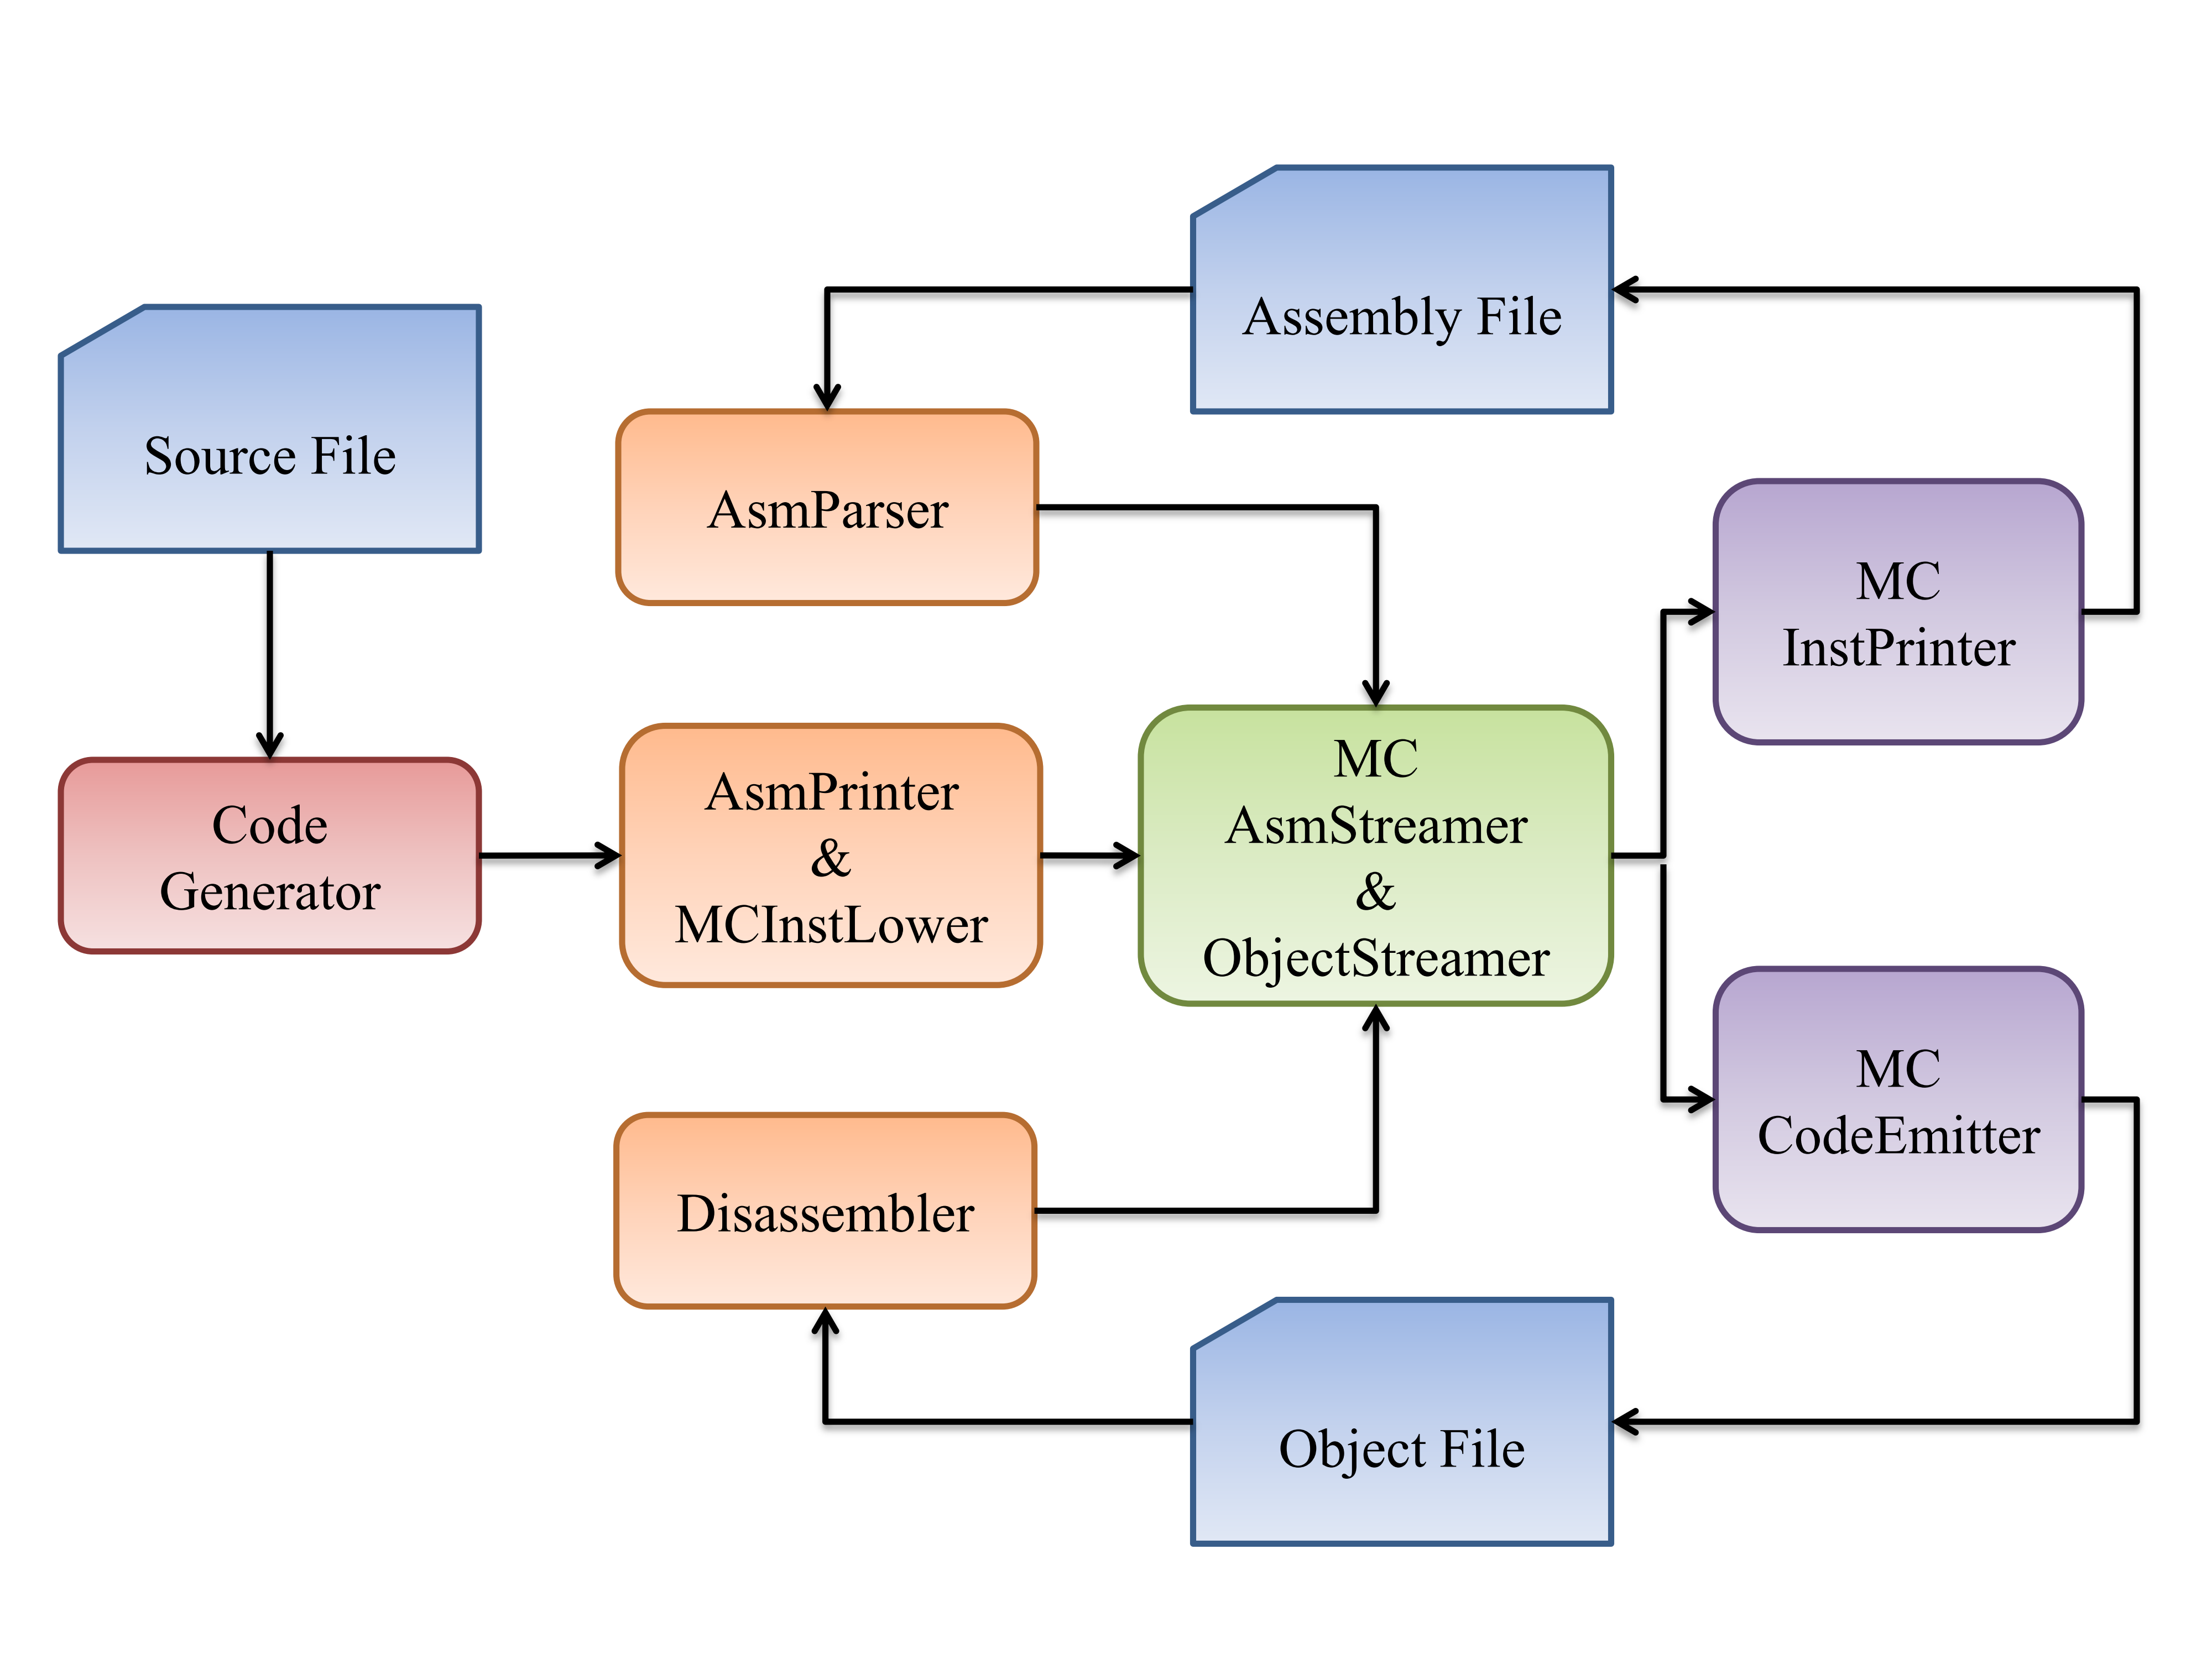
\includegraphics[scale=0.4]{fig/mc_layer_structure.png}
\end{figure}

\end{frame}

%----------- slide --------------------------------------------------%
\begin{frame}
  \frametitle{What Is The Role of MC?}

\begin{figure}
  \centering 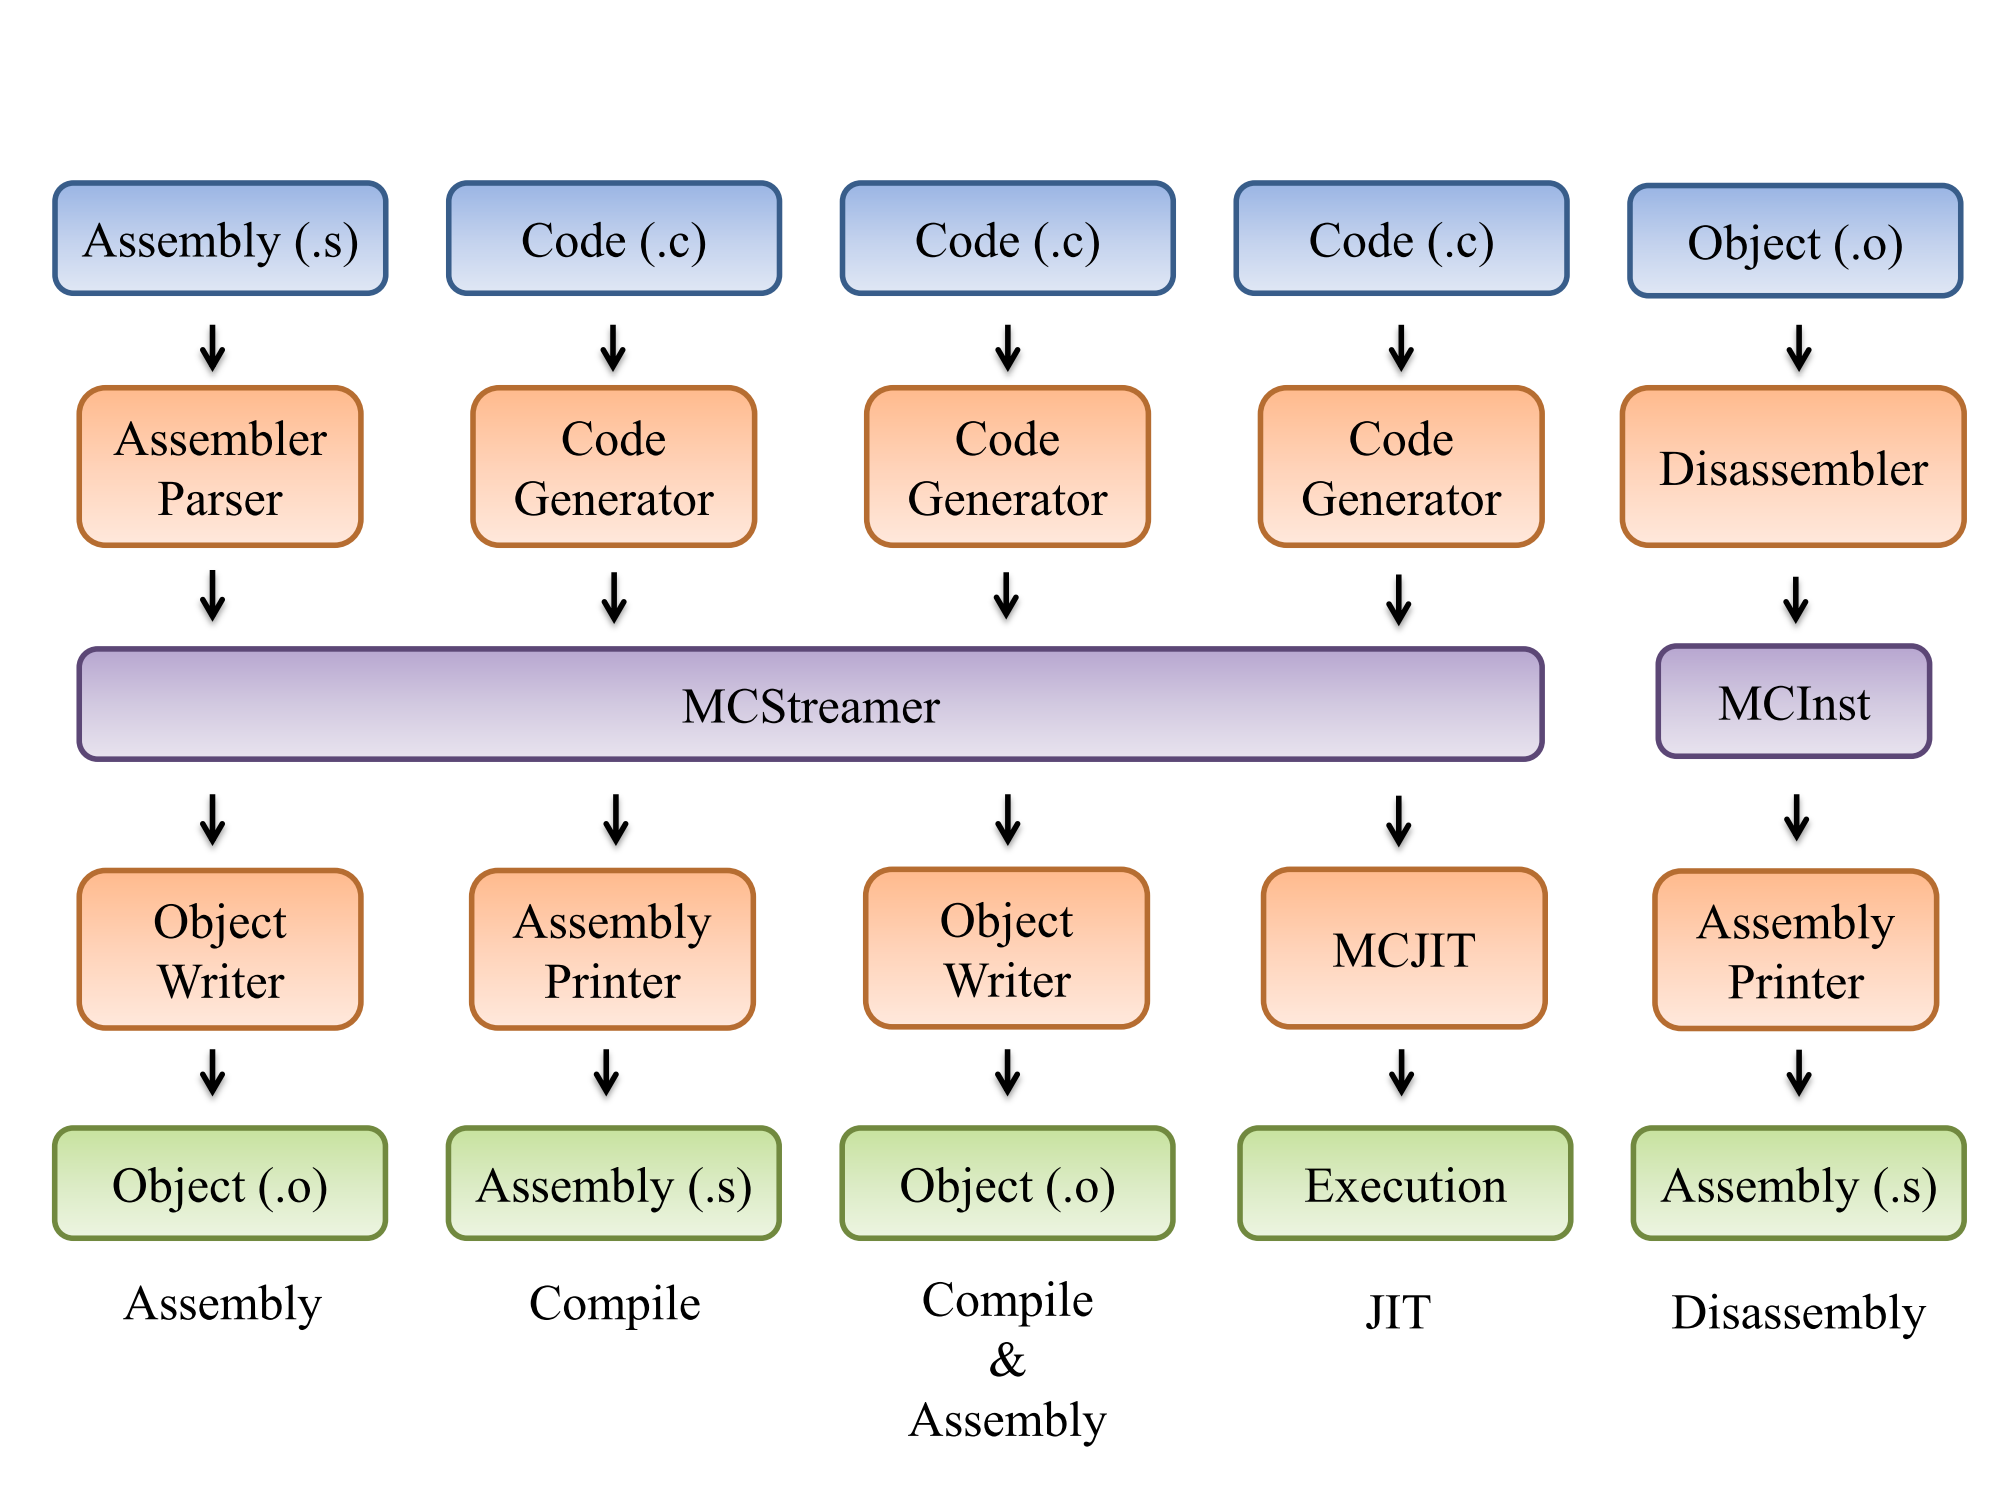
\includegraphics[scale=0.8]{fig/mcstreamer_and_mcinst.png}
\end{figure}

\end{frame}

%----------- slide --------------------------------------------------%
%\begin{frame}
%  \frametitle{What Is The Role of MC? 2/2}
%
%\begin{itemize}
%  \item MCStreamer: A C++ abstract base class aims to provide interface for
%  machine code emission.
%  \item MCAsmStreamer/MCObjectSteamer: They are implementation of MCStreamer
%  interface, prepare assembly/object file content ready for output.
%  \item MCInstPrinter/MCCodeEmitter: Write assembly/object file out.
%\end{itemize}
%
%
%\end{frame}

%----------- slide --------------------------------------------------%
\begin{frame}
  \frametitle{Assembler Relaxation}

Assmbler can adjust the instructions for two purposes:

\begin{itemize}
  \item Correctness: If the operand of instruction is out of bound, either
        expand the instruction or replace it by a longer one.
  \item Optimization: Replace expensive instruction with a cheaper one.
\end{itemize}

  \vspace\baselineskip

This process is called \textit{relaxation}.
\end{frame}

%----------- slide --------------------------------------------------%
\begin{frame}[fragile]
  \frametitle{Assembler Relaxation Example 1/4}

\begin{Verbatim}[commandchars=\\\{\}]
\PY{k}{extern} \PY{k+kt}{int} \PY{n+nf}{bar}\PY{p}{(}\PY{k+kt}{int}\PY{p}{)}\PY{p}{;}

\PY{k+kt}{int} \PY{n+nf}{foo}\PY{p}{(}\PY{k+kt}{int} \PY{n}{num}\PY{p}{)} \PY{p}{\PYZob{}}
  \PY{k+kt}{int} \PY{n}{t1} \PY{o}{=} \PY{n}{num} \PY{o}{*} \PY{l+m+mi}{17}\PY{p}{;}
  \PY{k}{if} \PY{p}{(}\PY{n}{t1} \PY{o}{\PYZgt{}} \PY{n}{bar}\PY{p}{(}\PY{n}{num}\PY{p}{)}\PY{p}{)}
    \PY{k}{return} \PY{n}{t1} \PY{o}{+} \PY{n}{bar}\PY{p}{(}\PY{n}{num}\PY{p}{)}\PY{p}{;}
  \PY{k}{return} \PY{n}{num} \PY{o}{*} \PY{n}{bar}\PY{p}{(}\PY{n}{num}\PY{p}{)}\PY{p}{;}
\PY{p}{\PYZcb{}}
\end{Verbatim}


  \vspace\baselineskip

\begin{Verbatim}[commandchars=\\\{\}]
\PY{n+nv}{\PYZdl{} }clang \PYZhy{}S \PYZhy{}O2 relax.c
\PY{n+nv}{\PYZdl{} }clang \PYZhy{}c relax.s
\PY{n+nv}{\PYZdl{} }objdump \PYZhy{}d relax.o
\end{Verbatim}

\end{frame}

%----------- slide --------------------------------------------------%
\begin{frame}[shrink=20]
  \frametitle{Assembler Relaxation Example 2/4}

\begin{Verbatim}[commandchars=\\\{\}]
\PY{l+m+mh}{0000000000000000} \PY{p}{\PYZlt{}}\PY{n+nf}{foo}\PY{p}{\PYZgt{}:}
  \PY{n+nl}{1a:}	\PY{l+m+mh}{e8 00 00 00 00 }      	\PY{n+nf}{callq}  \PY{l+m+mh}{1f} \PY{p}{\PYZlt{}}\PY{n+no}{foo}\PY{p}{+}\PY{l+m+mi}{0x1f}\PY{p}{\PYZgt{}}
  \PY{n+nl}{1f:}	\PY{l+m+mh}{45 39 f7 }            	\PY{n+nf}{cmp}    \PY{n+nv}{\PYZpc{}r14d}\PY{p}{,}\PY{n+nv}{\PYZpc{}r15d}
  \PY{n+nl}{22:}	\PY{l+m+mh}{7e 05 }               	\PY{n+nf}{jle}    \PY{l+m+mh}{29} \PY{p}{\PYZlt{}}\PY{n+no}{foo}\PY{p}{+}\PY{l+m+mi}{0x29}\PY{p}{\PYZgt{}}
  \PY{n+nl}{24:}	\PY{l+m+mh}{44 01 f8 }            	\PY{n+nf}{add}    \PY{n+nv}{\PYZpc{}r15d}\PY{p}{,}\PY{n+nv}{\PYZpc{}eax}
  \PY{n+nl}{27:}	\PY{l+m+mh}{eb 03 }               	\PY{n+nf}{jmp}    \PY{l+m+mh}{2c} \PY{p}{\PYZlt{}}\PY{n+no}{foo}\PY{p}{+}\PY{l+m+mi}{0x2c}\PY{p}{\PYZgt{}}
  \PY{n+nl}{29:}	\PY{l+m+mh}{0f af c3 }            	\PY{n+nf}{imul}   \PY{n+nv}{\PYZpc{}ebx}\PY{p}{,}\PY{n+nv}{\PYZpc{}eax}
  \PY{n+nl}{2c:}	\PY{l+m+mh}{48 83 c4 08 }         	\PY{n+nf}{add}    \PY{n+no}{\PYZdl{}0x8}\PY{p}{,}\PY{n+nv}{\PYZpc{}rsp}
  \PY{n+nl}{30:}	\PY{l+m+mh}{5b }                  	\PY{n+nf}{pop}    \PY{n+nv}{\PYZpc{}rbx}
  \PY{n+nl}{31:}	\PY{l+m+mh}{41 5e }               	\PY{n+nf}{pop}    \PY{n+nv}{\PYZpc{}r14}
  \PY{n+nl}{33:}	\PY{l+m+mh}{41 5f }               	\PY{n+nf}{pop}    \PY{n+nv}{\PYZpc{}r15}
  \PY{n+nl}{35:}	\PY{l+m+mh}{5d }                  	\PY{n+nf}{pop}    \PY{n+nv}{\PYZpc{}rbp}
  \PY{n+nl}{36:}	\PY{l+m+mh}{c3 }                  	\PY{n+nf}{retq}   
\end{Verbatim}


\end{frame}
%----------- slide --------------------------------------------------%
\begin{frame}[shrink=20]
  \frametitle{Assembler Relaxation Example 3/4}

% after

\begin{Verbatim}[commandchars=\\\{\}]
	\PY{n+nf}{callq}	\PY{n+no}{bar}
	\PY{n+nf}{cmpl}	\PY{n+nv}{\PYZpc{}r14d}\PY{p}{,} \PY{n+nv}{\PYZpc{}r15d}
	\PY{n+nf}{jle}	\PY{n+no}{.LBB0\PYZus{}2}
	\PY{n+na}{.fill} \PY{l+m+mi}{124}\PY{p}{,} \PY{l+m+mi}{1}\PY{p}{,} \PY{l+m+mi}{0x90} \PY{c}{\PYZsh{} nop}
\PY{c}{\PYZsh{} BB\PYZsh{}1:}
	\PY{n+nf}{addl}	\PY{n+nv}{\PYZpc{}r15d}\PY{p}{,} \PY{n+nv}{\PYZpc{}eax}
	\PY{n+nf}{jmp}	\PY{n+no}{.LBB0\PYZus{}3}
\PY{n+nl}{.LBB0\PYZus{}2:}
	\PY{n+nf}{imull}	\PY{n+nv}{\PYZpc{}ebx}\PY{p}{,} \PY{n+nv}{\PYZpc{}eax}
\PY{n+nl}{.LBB0\PYZus{}3:}
	\PY{n+nf}{addq}	\PY{n+no}{\PYZdl{}8}\PY{p}{,} \PY{n+nv}{\PYZpc{}rsp}
	\PY{n+nf}{popq}	\PY{n+nv}{\PYZpc{}rbx}
	\PY{n+nf}{popq}	\PY{n+nv}{\PYZpc{}r14}
	\PY{n+nf}{popq}	\PY{n+nv}{\PYZpc{}r15}
	\PY{n+nf}{popq}	\PY{n+nv}{\PYZpc{}rbp}
	\PY{n+nf}{ret}
\end{Verbatim}


\end{frame}

%----------- slide --------------------------------------------------%
\begin{frame}[shrink=20]
  \frametitle{Assembler Relaxation Example 4/4}

\begin{Verbatim}[commandchars=\\\{\}]
\PY{l+m+mh}{0000000000000000} \PY{p}{\PYZlt{}}\PY{n+nf}{foo}\PY{p}{\PYZgt{}:}
  \PY{n+nl}{1a:}	\PY{l+m+mh}{e8 00 00 00 00 }      	\PY{n+nf}{callq}  \PY{l+m+mh}{1f} \PY{p}{\PYZlt{}}\PY{n+no}{foo}\PY{p}{+}\PY{l+m+mi}{0x1f}\PY{p}{\PYZgt{}}
  \PY{n+nl}{1f:}	\PY{l+m+mh}{45 39 f7 }            	\PY{n+nf}{cmp}    \PY{n+nv}{\PYZpc{}r14d}\PY{p}{,}\PY{n+nv}{\PYZpc{}r15d}
  \PY{n+nl}{22:}	\PY{l+m+mh}{0f 8e 81 00 00 00 }   	\PY{n+nf}{jle}    \PY{l+m+mh}{a9} \PY{p}{\PYZlt{}}\PY{n+no}{foo}\PY{p}{+}\PY{l+m+mi}{0xa9}\PY{p}{\PYZgt{}}
  \PY{n+nl}{28:}	\PY{l+m+mh}{90 }                  	\PY{n+nf}{nop}
  \PY{n+nl}{a3:}	\PY{l+m+mh}{90 }                  	\PY{n+nf}{nop}
  \PY{n+nl}{a4:}	\PY{l+m+mh}{44 01 f8 }            	\PY{n+nf}{add}    \PY{n+nv}{\PYZpc{}r15d}\PY{p}{,}\PY{n+nv}{\PYZpc{}eax}
  \PY{n+nl}{a7:}	\PY{l+m+mh}{eb 03 }               	\PY{n+nf}{jmp}    \PY{l+m+mh}{ac} \PY{p}{\PYZlt{}}\PY{n+no}{foo}\PY{p}{+}\PY{l+m+mi}{0xac}\PY{p}{\PYZgt{}}
  \PY{n+nl}{a9:}	\PY{l+m+mh}{0f af c3 }            	\PY{n+nf}{imul}   \PY{n+nv}{\PYZpc{}ebx}\PY{p}{,}\PY{n+nv}{\PYZpc{}eax}
  \PY{n+nl}{ac:}	\PY{l+m+mh}{48 83 c4 08 }         	\PY{n+nf}{add}    \PY{n+no}{\PYZdl{}0x8}\PY{p}{,}\PY{n+nv}{\PYZpc{}rsp}
  \PY{n+nl}{b0:}	\PY{l+m+mh}{5b }                  	\PY{n+nf}{pop}    \PY{n+nv}{\PYZpc{}rbx}
  \PY{n+nl}{b1:}	\PY{l+m+mh}{41 5e }               	\PY{n+nf}{pop}    \PY{n+nv}{\PYZpc{}r14}
  \PY{n+nl}{b3:}	\PY{l+m+mh}{41 5f }               	\PY{n+nf}{pop}    \PY{n+nv}{\PYZpc{}r15}
  \PY{n+nl}{b5:}	\PY{l+m+mh}{5d }                  	\PY{n+nf}{pop}    \PY{n+nv}{\PYZpc{}rbp}
  \PY{n+nl}{b6:}	\PY{l+m+mh}{c3 }                  	\PY{n+nf}{retq}   
\end{Verbatim}


\end{frame}

%----------- slide --------------------------------------------------%
\begin{frame}
  \frametitle{Section and Fragment}

\begin{figure}
  \centering 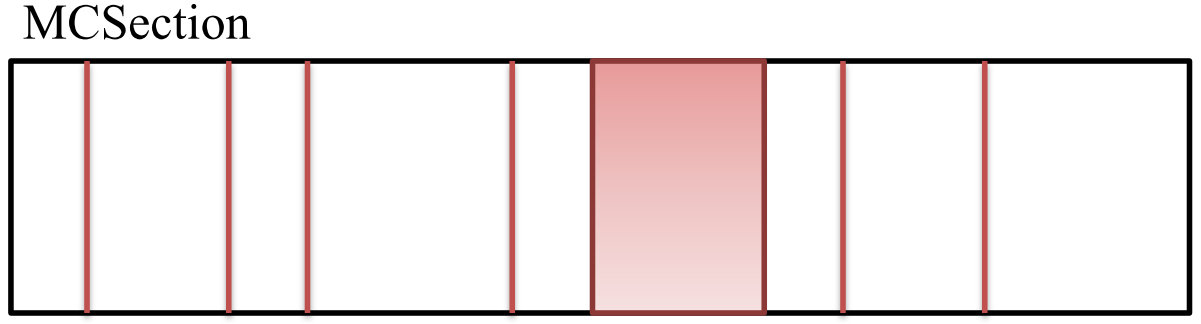
\includegraphics[scale=0.3]{fig/section_and_fragment_v1.png}
\end{figure}

In order to make relaxation process easier, LLVM keeps instructions as
a linked list of \textit{Fragment} not a byte array.

\begin{figure}
  \centering 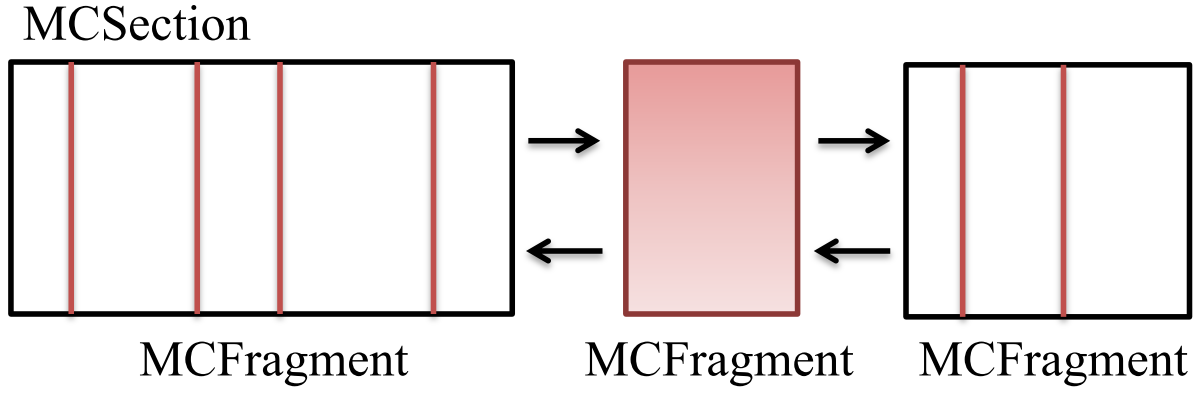
\includegraphics[scale=0.3]{fig/section_and_fragment_v2.png}
\end{figure}

\begin{itemize}
  \item MCAssembler::layoutSectionOnce (lib/MC/MCAssembler.cpp)
\end{itemize}

\end{frame}

%----------- slide --------------------------------------------------%
%\begin{frame}
%  \frametitle{Section and Fragment 2/2}
%
%\begin{enumerate}
%  \item Assembly directives and instructions are parsed, encoded and
%        collected into fragments.
%  \item Calculate the offsets of each fragments inside the section,
%        and start relaxation iteratively.
%  \item Fragments are written into a linear buffer for object file
%        emission.
%\end{enumerate}
%
%\end{frame}

%----------- slide --------------------------------------------------%
\begin{frame}
  \frametitle{Reference}

\begin{itemize}
  \item \href{http://www.hellogcc.org/download/hellogcc-2012.pdf}{LLVM - Another Toolchain Platform}
  \item \href{http://www.opus.ub.uni-erlangen.de/opus/volltexte/2010/1659/pdf/tricore_llvm.pdf}{Design and Implementation of a TriCore Backend for the LLVM Compiler Framework}
  \item \href{http://blog.llvm.org/2012/11/life-of-instruction-in-llvm.html}{Life of an instruction in LLVM}
  \item \href{http://eli.thegreenplace.net/2013/01/03/assembler-relaxation/}{Assembler relaxation}
  \item \href{http://mclinker.googlecode.com/files/instruction_relaxing.pdf}{Instruction Relaxation}
  \item \href{http://blog.llvm.org/2010/04/intro-to-llvm-mc-project.html}{Intro to the LLVM MC Project}
  \item \href{http://www.llvm.org/devmtg/2010-11/Dunbar-MC.pdf}{The LLVM Assembler \& Machine Code Infrastructure}
  \item \href{http://www.embecosm.com/appnotes/ean10/ean10-howto-llvmas-1.0.html}{Howto: Implementing LLVM Integrated Assembler}
  \item \href{http://www.aosabook.org/en/llvm.html}{The Architecture of Open Source Applications - Chapter LLVM}
  \item \href{http://llvm.org/docs/CodeGenerator.html}{The LLVM Target-Independent Code Generator}
\end{itemize}

\end{frame}

%----------- slide --------------------------------------------------%
\begin{frame}
  \frametitle{The End}

\centering{Q \& A}

\end{frame}

%----------- slide --------------------------------------------------%
\begin{frame}

\centering{You can download the \href{http://people.cs.nctu.edu.tw/~chenwj/slide/Talk/mclinker-2013/talk.txt}{manuscript}
and related material from \href{http://people.cs.nctu.edu.tw/~chenwj/slide/Talk/mclinker-2013/}{here}.}

\end{frame}

\end{CJK}
\end{document}
